% ============================================================================ %
%
%           Šablona bakalářské/diplomové práce
%
% Autor:    Ing. Jozef Říha (4. květen 2006)
%           (některé komentáře převzaty z dokumentu Ivana Pomykacze)
%
% Verze:    2017-01-19, Ing. Pavel Tomášek (tomasek@fai.utb.cz)
%
% Kódování: UTF-8 (žluťoučký kůň úpěl ďábelšké ódy)
%
% Sazba:    pdflatex prace.tex && pdflatex prace.tex
%           (nutné dvakrát pro korektní vložení citací a jiných referencí),
%           v případě umístění literatury do externího bib souboru je třeba volat
%           pdflatex statement.tex && bibtex statement.tex && pdflatex statement.tex && pdflatex statement.tex
%
% Tip:      Ve správně vysázeném českém textu by na konci řádku neměla zůstant
%           samotná jednopísmenná předložka. Na takové místo se vkládá
%           nezalomitelná mezera pomocí symbolu ~. Existuje program, který umí
%           zpracovat celý TeX dokument najednou podle českých konvencí:
%           http://petr.olsak.net/ftp/olsak/vlna/
%
%           Pozor! Vzhledem k požadovanému standardu PDF/A nesmí obrázky obsahovat 
%           alfa kanál (průhlednost).
%
% ============================================================================ %


\documentclass[a4paper,12pt]{article}

% Definice vzhledu a nastavení se načítá z následujícího souboru (netřeba editovat)
% ============================================================================ %
% Tento dokument není zpravidla třeba editovat,
% obsahuje nastavení balíčků, vzhledu, stylů.
%
% Kódování: UTF-8 (žluťoučký kůň úpěl ďábelšké ódy)
% ============================================================================ %


% ============================================================================ %
% BALÍČKY

%\usepackage[czech,english]{babel} % volba při kompilaci latexem (vyžaduje texlive-lang), zakomentovano, nastavovanu prikazem \nastavjazyk
\usepackage[T1]{fontenc}% definice vnitřního kódování
\usepackage[utf8x]{inputenc} % slouží pro definici kódování (při problémech zkusit zaměnit utf8x za utf8)
\usepackage{color}      % umožňuje použití barev
\usepackage{graphicx}	% rozšíření práce s grafikou
\usepackage{amsmath}	% balíček pro pokročilejší matematiku
\usepackage{fancyhdr}	% detailnější nastavení záhlaví a zápatí
\usepackage{tocloft}	% umožňuje pohodlné nastavení vzhledu obsahu, seznamu tabulek či obrázků
\usepackage{textcase}	% změna VeLiKoStI PíSmA
\usepackage{ifthen} 	% balíček umožňující skladby if, then -- využijeme při definici nadpisů
\usepackage{setspace}	% balíček umožňující nastavit řádkování na 1, 1.5, 2
\usepackage{ccaption}	% vylepšení práce s popisky obrázků či tabulek
\usepackage{sectsty}	% pro nastavení vzhledu nadpisů
\usepackage[srcstyle=leftnumhang,linenumbersep={\ }]{examplep} % pokročilejší sazba programového kódu
\usepackage{url}        % balíček pro vysázení internetové adresy stylem verbatim s vylepšeným řádkovým zlomem
\usepackage{afterpage}
%\usepackage{layout}	% zobrazí nastavení tiskového zrcadla (příkaz \layout)
%\usepackage{times}		% balíček pro použití fontu times
%\usepackage{verbatim}	% vysází text bez formátování, tak jak je zapsán v souboru
%\usepackage{indentfirst} % definuje odsazení prvního řádku odstavce
%\usepackage{makeidx}	% vytvoří rejstřík
\usepackage[pdftex,pdfa,hidelinks,breaklinks]{hyperref}	% vytváří křížové odkazy
%\usepackage{multicol}	% vícesloupcová sazba
%\usepackage{flafter}	% zajistí, aby se plovoucí objekty objevovali až za jejich umístěním v textu
\usepackage{chngcntr}   % Umožňuje změnu nastavení číslování obrázků, tabulek i rovnic
\usepackage{etoolbox}   % Tool-box for LaTeX programmers
\usepackage[labelsep=space,tableposition=bottom,justification=centering]{caption} % Přenastavení popisků u figur a tabulek

% --------------------------- Uživatelsky definované balíčky
\usepackage{framed} 	% Pro definice (Např. pro konečný automat)
\usepackage{ragged2e}	% Pro odsazení textu do leva (Např. například v definici konečného automatu)
\usepackage{amssymb}	% Pro specialní symboly, např. pro prazdnou mnozinu v algoritmu prevodu CFG na PDA
\usepackage{pdfpages}	% Pro vlozeni zadani v pdf
%\usepackage{tabularx}

% ---------------------------------------------------------------------------- %

\usepackage{xmpincl}
\usepackage{hyperxmp}

% \convertDate converts D:20080419103507+02'00' to 2008-04-19T10:35:07+02:00
\def\convertDate{%
    \getYear
}
{\catcode`\D=12
 \gdef\getYear D:#1#2#3#4{\edef\xYear{#1#2#3#4}\getMonth}
}
\def\getMonth#1#2{\edef\xMonth{#1#2}\getDay}
\def\getDay#1#2{\edef\xDay{#1#2}\getHour}
\def\getHour#1#2{\edef\xHour{#1#2}\getMin}
\def\getMin#1#2{\edef\xMin{#1#2}\getSec}
\def\getSec#1#2{\edef\xSec{#1#2}\getTZh}
\def\getTZh +#1#2{\edef\xTZh{#1#2}\getTZm}
\def\getTZm '#1#2'{%
    \edef\xTZm{#1#2}%
    \edef\convDate{\xYear-\xMonth-\xDay T\xHour:\xMin:\xSec+\xTZh:\xTZm}%
}
\expandafter\convertDate\pdfcreationdate

\pdfminorversion 4

\immediate\pdfobj stream attr{/N 3}  file{graphics/sRGBIEC1966-2.1.icm}
\pdfcatalog{%
  /OutputIntents [ <<
  /Type /OutputIntent
  /S/GTS_PDFA1
  /DestOutputProfile \the\pdflastobj\space 0 R
  /OutputConditionIdentifier (sRGB IEC61966-2.1)
  /Info(sRGB IEC61966-2.1)
 >> ]
}

\providecommand{\xmpOrg}{Tomas Bata University in Zlín, Czech Republic}
\providecommand{\xmpProducer}{}
\providecommand{\xmpDoi}{}
\providecommand{\xmpJournalnumber}{}
\providecommand{\xmpVolume}{}
\providecommand{\xmpIssue}{}
\providecommand{\xmpCoverDisplayDate}{}
\providecommand{\xmpCoverDate}{}
\providecommand{\xmpJournaltitle}{}
\providecommand{\xmpFirstpage}{}
\providecommand{\xmpLastpage}{}
\providecommand{\xmpAuthoritativeDomain}{}
\providecommand{\xmpCreatorTool}{}


% ============================================================================ %
% NASTAVENÍ TISKOVÉHO ZRCADLA

\newcommand{\valueTextHeight}{242mm}	% výška tiskového zrcadla
\newcommand{\valueTextWidth}{155mm}	% šířka tiskového zrcadla
\newcommand{\valueVOffset}{-1.61cm}	% vertikální posunutí tiskového zrcadla
\newcommand{\valueSideMargin}{0.96cm}	% levý okraj
\newcommand{\valueHeadHeight}{0.6cm}	% záhlaví
\newcommand{\valueHeadSep}{1cm}	% záhlaví

\textheight=\valueTextHeight
\textwidth=\valueTextWidth
\voffset=\valueVOffset
%\voffset=-1in
%\topmargin=-2.9cm

\oddsidemargin=\valueSideMargin
\evensidemargin=\valueSideMargin

\headheight=\valueHeadHeight
\headsep=\valueHeadSep

% nastavení zápatí
\footskip=1ex
\cfoot{}
% "vypnout" poznámky na okrajích
\marginparpush=0mm
\marginparwidth=0mm
\marginparsep=0mm

\pagestyle{fancy}

% Nastavení obalujících okrajů okolo popisků figur a tabulek
\captionsetup[figure]{aboveskip=10pt}
\captionsetup[figure]{belowskip=0pt}
\captionsetup[table]{aboveskip=0pt}
\captionsetup[table]{belowskip=-5pt}


% ============================================================================ %
% NASTAVENÍ PÍSMA, ODSTAVCE, ROVNIC, POZNÁMEK

\parindent=0em				% velikost odstavcové zarážky na nulu
\def\thefootnote{\arabic{footnote})}	% poznámka pod čarou se závorkou
\onehalfspacing % nastavím řádkování tímto způsobem nebo \renewcommand{\baselinestretch}{1.5} ??
\setlength{\parskip}{3pt}		% vertikální mezera mezi nadpisy
%\def\label#1{{\sf ! #1 ! }}		% možnost zobrazení všech \label{}


% ============================================================================ %
% NASTAVENÍ ČÍTAČŮ

\setcounter{tocdepth}{3} % do obsahu se ukládají pouze první dvě úrovně kapitol


% ============================================================================ %
% PDF/A STANDARD

% http://www.mathstat.dal.ca/~selinger/pdfa/
% https://blog.zhaw.ch/icclab/creating-pdfa-documents-for-long-term-archiving/
% http://support.river-valley.com/wiki/index.php?title=Generating_PDF/A_compliant_PDFs_from_pdftex

% Prerequisites: pdflatex, hyperref, xmpincl
% pdfTeX at least in version 1.40.15 (in Linux add repository ppa:jonathonf/texlive, update and upgrade texlive-full)
%
% Validator: https://www.pdf-online.com/osa/validate.aspx

\newcommand{\aplikujpdfa}{
	\ifczech
		\providecommand{\xmpTitle}{\nazevcz}
		\providecommand{\xmpAuthor}{\autor}
		\providecommand{\xmpKeywords}{\klicovaslovacz}
		\hypersetup{
			pdftitle={\nazevcz},
			pdfauthor={\autor},
			pdfsubject={\abstraktcz},
			pdfkeywords={\klicovaslovacz},
			pdflang={en}
		}
	\else \ifenglish
		\providecommand{\xmpTitle}{\nazeven}
		\providecommand{\xmpAuthor}{\autor}
		\providecommand{\xmpKeywords}{\klicovaslovaen}
		\hypersetup{
			pdftitle={\nazeven},
			pdfauthor={\autor},
			pdfsubject={\abstrakten},
			pdfkeywords={\klicovaslovaen},
			pdflang={en}
		}
	\fi \fi
	
	\makeatletter
	\includexmp{tex/pdfa-1b}
	\makeatother
}


% ============================================================================ %
% UŽIVATELSKÉ STYLY

% Styl nn = nečíslovaný nadpis (je vysázený v obsahu)
\def\nn#1{\clearpage\section*{\MakeTextUppercase{#1}}\addcontentsline{toc}{section}{#1}}

% Styl nm = nečíslovaný nadpis (není vysázený v obsahu)
\def\nm#1{\clearpage\section*{\MakeTextUppercase{#1}}}

% Styl ns = nečíslovaný nadpis na stejné stránce (není vysázený v obsahu)
\def\nns#1{\section*{\MakeTextUppercase{#1}}}

% Styl n{ur}{nadp} pro nadpisy, kde ur je číslo úrovně a nadp je text nadpisu
\def\n#1#2{
	\ifthenelse{#1=1}{\clearpage\section{#2}}{
		\ifthenelse{#1=2}{\subsection{#2}}{
			\ifthenelse{#1=3}{\subsubsection{#2}}{\paragraph{\itshape\bfseries{#2}}
}}}}

% Styl pro obrázky
% \obr{popisek}{label}{rozměr (0.0 - 1.0)}{soubor}
\def\obr#1#2#3#4{
	\begin{figure}[h]
		\centering
		\includegraphics[width=#3\linewidth]{#4}
		%\captionwidth{#3\linewidth}
		%\changecaptionwidth
		\captionsetup{width=#3\linewidth}
		\caption{#1}
		\label{#2}
	\end{figure}
}

% Styl pro tabulky
% \tab{popisek}{label}{rozměr (0.0 - 1.0)}{definice sloupců}{obsah} 
\def\tab#1#2#3#4#5{
	\begin{table}[h]
		%\captionwidth{#3\linewidth}
		%\changecaptionwidth
		\captionsetup{width=#3\linewidth}
		\caption{#1}
		\label{#2}
		\begin{center}
			\centering
			\begin{tabular}{#4}
				#5
			\end{tabular}
		\end{center}
	\end{table}
}

% Styl pro tabulky v příloze
% \tabpri{popisek}{definice sloupců}{data tabulky}
\def\tabpri#1#2#3{
	\begin{table}[h]
	\begin{center}
	#1
	\end{center}
	\begin{center}
	\begin{tabular}{#2}
	#3
	\end{tabular}
	\end{center}
	\end{table}
}
	
% Styl pro tabulky z MS Excelu exportované do EPS
% \extab{popisek}{rozměr (0.0 - 1.0)}{soubor}
\def\extab#1#2#3{
	\begin{table}
	%\captionwidth{#2\linewidth}
	%\changecaptionwidth
	\captionsetup{width=#2\linewidth}
	\caption{#1}
	\begin{center}
	\includegraphics[width=#2\linewidth]{#3}
	\end{center}
	\end{table}
}

% Styl pro rovnice
% \rov[klíčové slovo]{rovnice}
\newcommand{\rov}[2][chybejici rovnice]{
	\begin{equation}
	#2
	\label{#1}
	\end{equation}
}
	
% Příkaz pro vysázení seznamu obrázků
\def\seznamobr{
	\clearpage
	\ifczech
		\addcontentsline{toc}{section}{Seznam obrázků}
	\else \ifenglish
		\addcontentsline{toc}{section}{List of Figures}
	\fi \fi
	\listoffigures
	\clearpage
}

% Příkaz pro vysázení seznamu tabulek
\def\seznamtab{
	\clearpage
	\ifczech
		\addcontentsline{toc}{section}{Seznam tabulek}
	\else \ifenglish
		\addcontentsline{toc}{section}{List of Tables}
	\fi \fi
	\listoftables
	\clearpage
}

\newcommand{\OdsazovaniOdstavcuStart}[0]{
	\ifenglish
		\setlength{\parskip}{5mm} % English indentation of paragraphs
	\else \ifczech
		\setlength{\parindent}{5mm} % Czech indentation of paragraphs
	\fi \fi
}

\newcommand{\OdsazovaniOdstavcuStop}[0]{
	\ifenglish
		\setlength{\parskip}{0mm} % English indentation of paragraphs
	\else \ifczech
		\setlength{\parindent}{0mm} % Czech indentation of paragraphs
	\fi \fi
}

% Příkaz pro vysázení seznamu literatury
\newcommand{\seznamlit}[1]{
	\clearpage
	\ifczech
		\addcontentsline{toc}{section}{Seznam použité literatury}
	\else \ifenglish
		\addcontentsline{toc}{section}{References}
	\fi \fi
	\begin{thebibliography}{99}
	#1
	\end{thebibliography}
}

\newcommand{\seznamlitbib}{
	\bibliographystyle{tex/csplainnat} % Respects the norm of ČSN ISO 690
	\newpage
	\clearpage
	%\cleardoublepage
	\addcontentsline{toc}{section}{\protect\numberline{}{\ifenglish References \else \ifczech Seznam použité literatury \fi \fi}}
	\bibliography{tex/literatura}
}

% Příkaz pro přípravu seznamu použitých zkratek a symbolů
\newcommand{\seznamzkr}{
	\ifczech
		\nn{Seznam použitých symbolů a zkratek}
	\else \ifenglish
		\nn{List of Abbreviations}
	\fi \fi
}

% Příkaz \cast jako alternativa k \part
\def\cast#1{
	\part{#1}
}

% Příkaz \obsah vysází obsah v daném místě
\def\obsah{
	\deaktivujZahlavi
	\clearpage
	\thispagestyle{empty}
	\tableofcontents
	\clearpage
	\pagestyle{fancy}
	\aktivujZahlavi
}

% Zkrácení stylu \textbf na \b
\def\b#1{
	\textbf{#1}
}

% \bi = tučná kurzíva
\newcommand{\bi}[1]{\textbf{\textit{#1}}}

% \it = kurzíva
\renewcommand{\it}[1]{\textit{#1}}

% Nastaveni nezobrazovani zahlavi dokumentu
\newcommand{\deaktivujZahlavi}{
	\lhead{}
	\rhead{}
	\renewcommand{\headrulewidth}{0pt}
}

\newcommand{\zadani}{
	%\deaktivujZahlavi
	
	
		%\clearpage
		%\thispagestyle{empty}
		\voffset=\valueVOffset\evensidemargin=\valueSideMargin\oddsidemargin=\valueSideMargin\headsep=\valueHeadSep\headheight=\valueHeadHeight\setlength{\parskip}{3pt}\textheight=\valueTextHeight\textwidth=\valueTextWidth
		%*** Nascanované zadání, strana 1 ***
	
		%\clearpage
		%\thispagestyle{empty}
		%*** Nascanované zadání, strana 2 ***
		
		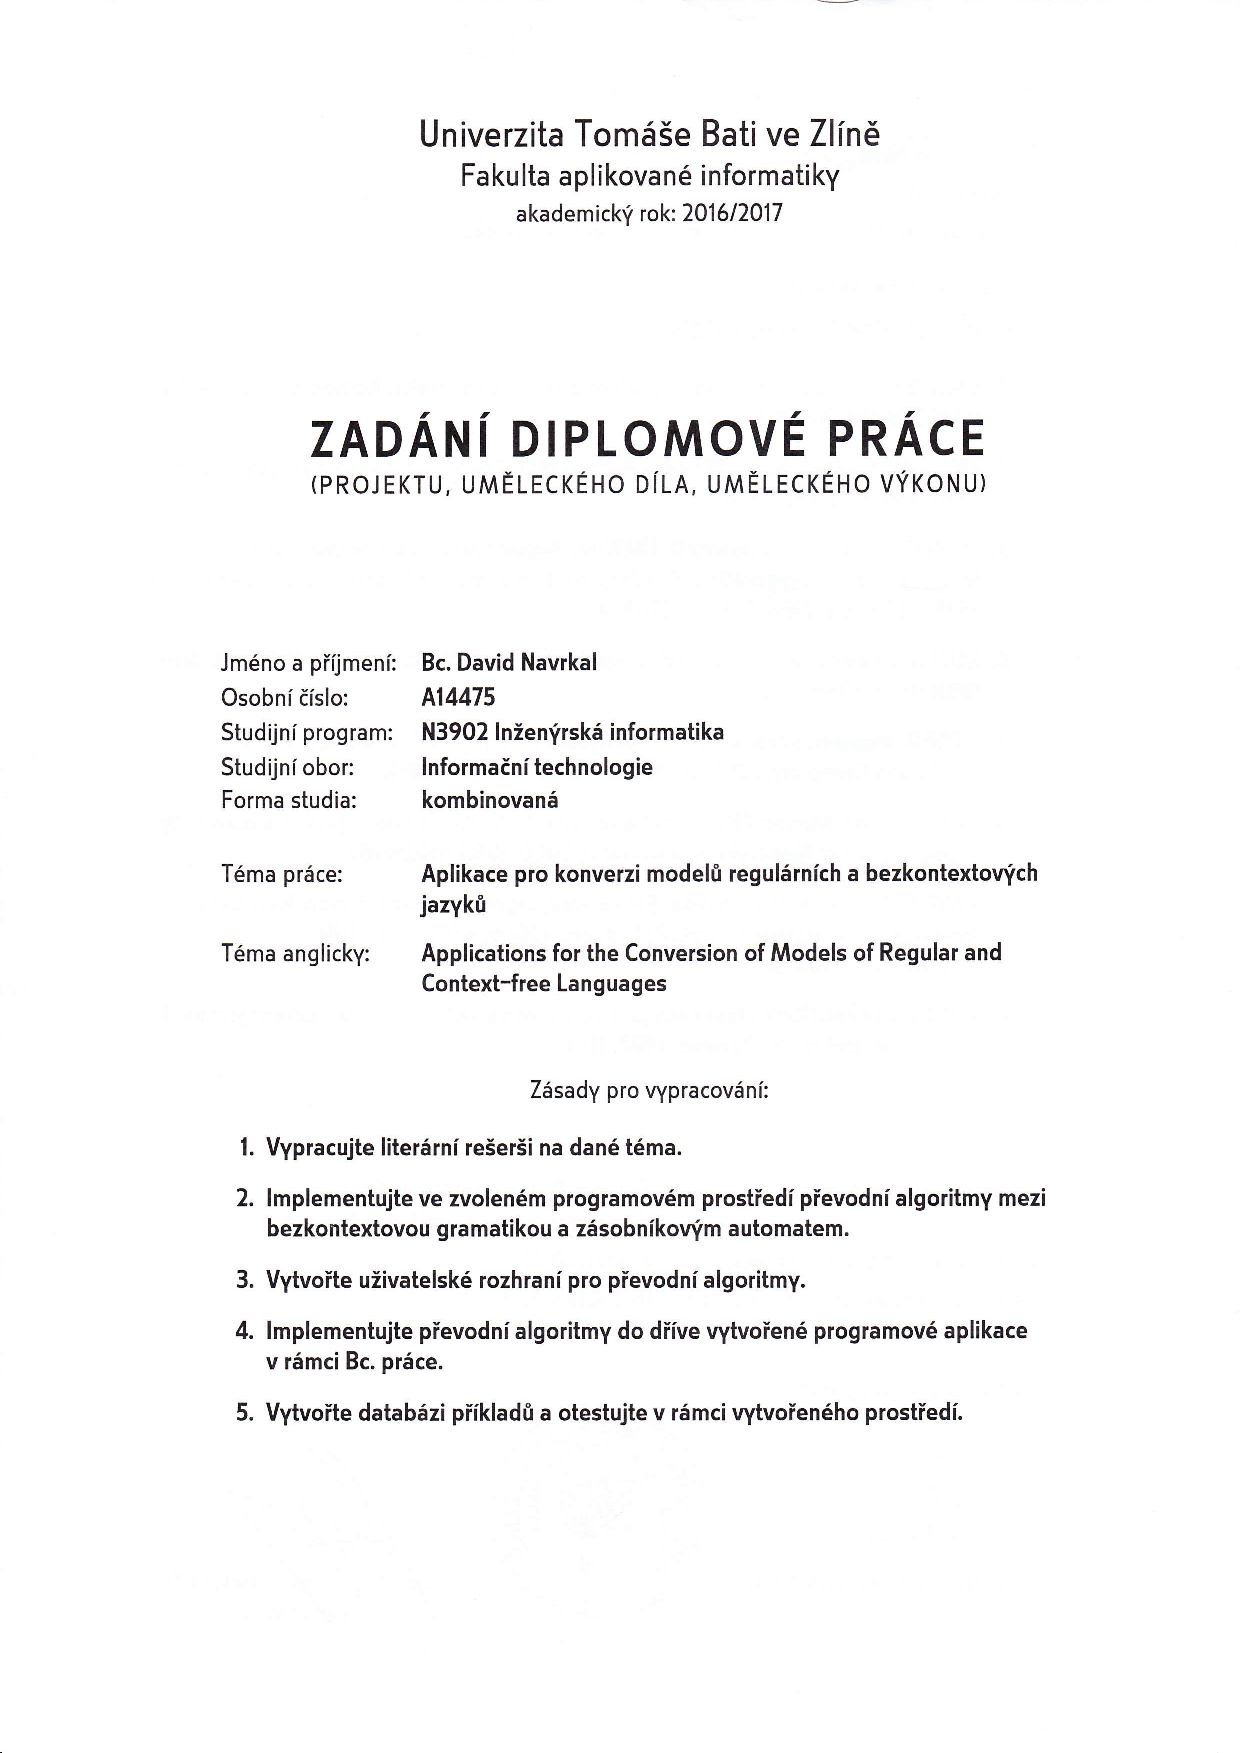
\includepdf[pages={1,2}]{zadani.pdf}
}

% Nastaveni zobrazovani zahlavi dokumentu
\newcommand{\aktivujZahlavi}{
	\renewcommand{\headrulewidth}{1pt}
	\rhead{\thepage}
	
	\ifczech
		\lhead{\b{UTB ve Zlíně, \ifthenelse{\equal{\fakulta}{FAI}}{Fakulta aplikované informatiky}{\ifthenelse{\equal{\fakulta}{FAME}}{Fakulta managementu a ekonomiky}{\ifthenelse{\equal{\fakulta}{FHS}}{Fakulta humanitních studií}{\ifthenelse{\equal{\fakulta}{FLKR}}{Fakulta logistiky a krizového řízení}{\ifthenelse{\equal{\fakulta}{FMK}}{Fakulta multimediálních komunikací}{\ifthenelse{\equal{\fakulta}{FT}}{Fakulta technologická}{\ifthenelse{\equal{\fakulta}{UNI}}{Univerzitní institut}{}}}}}}}}}
	\else \ifenglish
		\lhead{\b{TBU in Zlín, \ifthenelse{\equal{\fakulta}{FAI}}{Faculty of Applied Informatics}{\ifthenelse{\equal{\fakulta}{FAME}}{Faculty of Management and Economics}{\ifthenelse{\equal{\fakulta}{FHS}}{Faculty of Humanities}{\ifthenelse{\equal{\fakulta}{FLKR}}{Faculty of Logistics and Crisis Management}{\ifthenelse{\equal{\fakulta}{FMK}}{Faculty of Multimedia Communications}{\ifthenelse{\equal{\fakulta}{FT}}{Faculty of Technology}{\ifthenelse{\equal{\fakulta}{UNI}}{University Institute}{}}}}}}}}}
	\fi \fi
}

% Příkaz \logopracerok vloží na dané místo logo fakulty, typ práce a rok
\newcommand{\logopracerok}{
	\ifczech
		\iffai  \put(82.2,-223.3){\makebox(84,16.4){
\includegraphics[width=90mm]{graphics/logo/fai_logo_cz.png}}} \fi
		\iffame \put(82.2,-223.3){\makebox(84,16.4){
\includegraphics[width=90mm]{graphics/logo/fame_logo_cz.png}}} \fi
		\iffhs  \put(82.2,-223.3){\makebox(84,16.4){
\includegraphics[width=90mm]{graphics/logo/fhs_logo_cz.png}}} \fi
		\ifflkr \put(82.2,-223.3){\makebox(84,16.4){
\includegraphics[width=90mm]{graphics/logo/flkr_logo_cz.png}}} \fi
		\iffmk  \put(82.2,-223.3){\makebox(84,16.4){
\includegraphics[width=90mm]{graphics/logo/fmk_logo_cz.png}}} \fi
		\ifft   \put(82.2,-223.3){\makebox(84,16.4){
\includegraphics[width=90mm]{graphics/logo/ft_logo_cz.png}}} \fi
		\ifuni  \put(82.2,-223.3){\makebox(84,16.4){
\includegraphics[width=90mm]{graphics/logo/uni_logo_cz.png}}} \fi
	\else \ifenglish
		\iffai  \put(82.2,-223.3){\makebox(84,16.4){
\includegraphics[width=90mm]{graphics/logo/fai_logo_en.png}}} \fi
		\iffame \put(82.2,-223.3){\makebox(84,16.4){
\includegraphics[width=90mm]{graphics/logo/fame_logo_en.png}}} \fi
		\iffhs  \put(82.2,-223.3){\makebox(84,16.4){
\includegraphics[width=90mm]{graphics/logo/fhs_logo_en.png}}} \fi
		\ifflkr \put(82.2,-223.3){\makebox(84,16.4){
\includegraphics[width=90mm]{graphics/logo/flkr_logo_en.png}}} \fi
		\iffmk  \put(82.2,-223.3){\makebox(84,16.4){
\includegraphics[width=90mm]{graphics/logo/fmk_logo_en.png}}} \fi
		\ifft   \put(82.2,-223.3){\makebox(84,16.4){
\includegraphics[width=90mm]{graphics/logo/ft_logo_en.png}}} \fi
		\ifuni  \put(82.2,-223.3){\makebox(84,16.4){
\includegraphics[width=90mm]{graphics/logo/uni_logo_en.png}}} \fi
	\fi \fi
	\put(0,-205){\linethickness{1pt}\line(1,0){170}}
	\ifczech
		\ifbp \put(4,-215){\makebox(69.5,4.5)[l]{\noindent\fontsize{16}{1}\usefont{OT1}{phv}{m}{n}Bakalářská práce}} \fi
		\ifdp \put(4,-215){\makebox(69.5,4.5)[l]{\noindent\fontsize{16}{1}\usefont{OT1}{phv}{m}{n}Diplomová práce}} \fi
	\else \ifenglish
		\ifbp \put(4,-215){\makebox(69.5,4.5)[l]{\noindent\fontsize{16}{1}\usefont{OT1}{phv}{m}{n}Bachelor's thesis}} \fi
		\ifdp \put(4,-215){\makebox(69.5,4.5)[l]{\noindent\fontsize{16}{1}\usefont{OT1}{phv}{m}{n}Master's thesis}} \fi
	\fi \fi
	\put(4,-220){\makebox(69.5,4.5)[l]{\noindent\fontsize{16}{1}\usefont{OT1}{phv}{m}{n}\rok}}
	\put(0,-225){\linethickness{1pt}\line(1,0){170}}
	\put(75,-223.3){\linethickness{1pt}\line(0,1){16.4}}
}

% Úvodní stránka s logem fakulty
\newcommand{\titulnistrana}{
	\thispagestyle{empty}
	\voffset=-2.01cm\evensidemargin=0pt\oddsidemargin=0cm\parindent=0pt\headsep=0pt\headheight=0pt\parskip=0pt\textheight=272mm\textwidth=200mm
	\renewcommand{\baselinestretch}{0}
	
	\setlength{\unitlength}{1mm}
	\begin{picture}(-10,8)
		\ifczech
			% Nazev prace
			%\put(0,-100){\makebox(170,50){\fontsize{24}{1}\usefont{OT1}{phv}{b}{n}#1}}
			%		\put(0,-100){\makebox(170,50){\protect\parbox{0.8\textwidth}{\protect\centering\fontsize{24}{1}\usefont{OT1}{phv}{b}{n}#1}}}
			
			% Vyreseno odradkovani
			\put(0,-100){\makebox(170,50){\protect\parbox{0.8\textwidth}{\protect\centering\setstretch{2.0}\usefont{OT1}{phv}{b}{n}{\Huge\nazevcz}}}}
			
			% Jmeno autora
			\put(0,-135){\makebox(170,25){\fontsize{20}{1}\usefont{OT1}{phv}{m}{n}\autor}}
		\else \ifenglish
			% Nazev prace
			%\put(0,-100){\makebox(170,50){\fontsize{24}{1}\usefont{OT1}{phv}{b}{n}#1}}
			%\put(0,-95){\makebox(170,50){\protect\parbox{0.8\textwidth}{\protect\centering\fontsize{24}{1}\usefont{OT1}{phv}{b}{n}#1}}}
			\put(0,-88){\makebox(170,50){\protect\parbox{0.8\textwidth}{\protect\centering\setstretch{2.0}\usefont{OT1}{phv}{b}{n}{\Huge\nazeven}}}}
	
			%\put(0,-111){\makebox(170,50){\fontsize{20}{1}\usefont{OT1}{phv}{m}{n}#1}}
			%\put(0,-116){\makebox(170,50){\protect\parbox{0.8\textwidth}{\protect\centering\fontsize{20}{1}\usefont{OT1}{phv}{m}{n}#2}}}
			\put(0,-115){\makebox(170,50){\protect\parbox{0.8\textwidth}{\protect\centering\setstretch{1.5}\usefont{OT1}{phv}{m}{n}{\Large\nazevcz}}}}
			
			% Jmeno autora
			\put(0,-140){\makebox(170,25){\fontsize{20}{1}\usefont{OT1}{phv}{m}{n}\autor}}
		\fi \fi
		\logopracerok
	\end{picture}
}


% Strana s abstraktem a klíčovými slovy v češtině a angličtině
\newcommand{\abstraktaklicovaslova}{
	\clearpage
	\thispagestyle{empty}
	\nm{Abstrakt}
	\abstraktcz
	
	\vspace{1cm}
	Klíčová slova: \klicovaslovacz
	
	\vspace{3cm}
	
	\nns{Abstract}
	\abstrakten
	
	\vspace{1cm}
	Keywords: \klicovaslovaen
}

% Formatovani nonterminalu v definici Backus-Naurov formy
\newcommand{\nonTerm}[1] {\textbf{\textless #1\textgreater}}


% ============================================================================ %
% NASTAVENÍ ZOBRAZENÍ PŘÍLOH -- SEZNAM, ČÍSLOVÁNÍ, VLASTNÍ STYL

\makeatletter % tímto příkazem dávám najevo, že budu editovat přímo příkazy ze šablony

% definice seznamu příloh - příkaz \listofappendices
\def\listofappendices{%
	\newpage
	\setcounter{section}{0}
	\ifczech
		\addcontentsline{toc}{section}{SEZNAM PŘÍLOH}
		\@restonecolfalse\if@twocolumn\@restonecoltrue\onecolumn\fi
		\section*{SEZNAM PŘÍLOH}
	\else \ifenglish
		\addcontentsline{toc}{section}{LIST OF APPENDICES}
		\@restonecolfalse\if@twocolumn\@restonecoltrue\onecolumn\fi
		\section*{LIST OF APPENDICES}
	\fi \fi
	\@mkboth{LIST OF APPENDICES}{LIST OF APPENDICES}
	\@starttoc{loa}\if@restonecol\twocolumn\fi
	\pagestyle{empty}
	\thispagestyle{fancy}
}

\def\ext@appendix{loa}
\def\tocname{loa}

% definice příkazu \priloha{nazev prilohy} pro vložení nové přílohy
\newcommand{\priloha}[1]{
	\clearpage
	\refstepcounter{section}
	%\voffset=-3cm  % vertikalni posun
	\addtocontents{loa}{\protect\makebox[1.5cm][l]{P \@Roman\c@section.} #1\newline}
	\ifczech
		{\bf PŘÍLOHA P \@Roman\c@section. \MakeTextUppercase{#1}}
	\else \ifenglish
		{\bf APPENDIX P \@Roman\c@section. \MakeTextUppercase{#1}}
	\fi \fi
	\par
}

% ============================================================================ %
% OBSAH: NASTAVENÍ VELKÝCH PÍSMEN PRO NÁZVY SEKCÍ A HLAVNÍCH NADPISŮ

\let\oldcontentsline\contentsline
\def\contentsline#1#2{%
  \expandafter\ifx\csname l@#1\endcsname\l@section
    \expandafter\@firstoftwo
  \else
    \expandafter\@secondoftwo
  \fi
  {%
    \oldcontentsline{#1}{\MakeTextUppercase{#2}}%
  }{%
    \oldcontentsline{#1}{#2}%
  }%
}

\def\@part[#1]#2{
	\ifnum \c@secnumdepth >\m@ne
		\refstepcounter{part}
		\addcontentsline{toc}{section}{\protect\makebox[0.85cm]{\thepart\hfill} #1}
	\else
		\addcontentsline{toc}{section}{#1}
	\fi
	{\parindent \z@ \raggedright
	\interlinepenalty \@M
	\clearpage
	\normalfont
    \ifnum \c@secnumdepth >\m@ne
    	\Large\bfseries
		\nobreak
	\fi
	\vspace*{9cm}
	\center\huge \bfseries\thepart. \MakeTextUppercase{#2}
	\markboth{}{}\par}
	\nobreak
	\clearpage
    \@afterheading
}


% ============================================================================ %
% NASTAVENÍ FORMÁTU ČÍSLOVÁNÍ OBRÁZKŮ A TABULEK

\def\thefigure{\arabic{figure}}      % číslování obrázků typu (y)
\def\thetable{\arabic{table}}        % číslování tabulek typu (y)
\captiondelim{. } % změníme dvoutečku za Obr/Tab za tečku

% Nastavení číslování obrázků, tabulek i rovnic do formátu <číslo kapitoly>.<pořadové číslo>
\counterwithin{figure}{section}
\counterwithin{table}{section}
\counterwithin{equation}{section}

% Odsazeni popisku v seznamu obrazku a tabulek
\patchcmd{\@caption}{\csname the#1\endcsname}{\csname fnum@#1\endcsname}{}{}
%{\renewcommand*\numberline[1]{Fig. \,#1\space}}
\renewcommand*\l@figure{\@dottedtocline{1}{0em}{5.0em}}
\renewcommand*\l@table{\@dottedtocline{1}{0em}{5.0em}}

% Vynulování čítačů
\@addtoreset{table}{section}
\@addtoreset{figure}{section}
\@addtoreset{footnote}{section}
	
\makeatother % a to je ukončení \makeatletter


% ============================================================================ %
% ÚPRAVA VZHLEDU OBSAHU, SEZNAMU OBRÁZKŮ A TABULEK

% nastavení vertikální mezery před stylem část, nadpis 1--3
\setlength{\cftbeforepartskip}{3pt}
\setlength{\cftbeforesecskip}{3pt}
\setlength{\cftbeforesubsecskip}{3pt}
\setlength{\cftbeforesubsubsecskip}{0cm}

% odsazení zleva pro styl část, nadpis 1--3
\setlength{\cftpartindent}{0cm}
\setlength{\cftsecindent}{0cm}
\setlength{\cftsubsecindent}{0cm}
\setlength{\cftsubsubsecindent}{0cm}

% nastavení fontu pro styl část, nadpis 1--3
\renewcommand{\cftpartfont}{\small\bfseries}
\renewcommand{\cftsecfont}{\small\bfseries}
\renewcommand{\cftsubsecfont}{\scshape}
\renewcommand{\cftsubsubsecfont}{}

% odsazení čísla a textu titulku pro styl část, nadpis 1--3
\cftsetindents{part}{0cm}{1cm}
\cftsetindents{sec}{0cm}{1cm}
\cftsetindents{subsec}{0.5cm}{1.25cm}
\cftsetindents{subsubsec}{1cm}{1.5cm}
\cftsetindents{fig}{0cm}{1.5cm}
\cftsetindents{tab}{0cm}{1.5cm}

% nastavení vodící čáry pro styl část, nadpis 1--3, obrázky a tabulky
\renewcommand{\cftdot}{\ensuremath{.}} % tímto příkazem lze změnit vodící tečky v obsahu na jiný znak
\renewcommand{\cftpartleader}{\cftdotfill{0.3}}
\renewcommand{\cftsecleader}{\cftdotfill{0.3}}
\renewcommand{\cftsubsecleader}{\cftdotfill{0.3}}
\renewcommand{\cftsubsubsecleader}{\cftdotfill{0.3}}
\renewcommand{\cftfigleader}{\cftdotfill{0.3}}
\renewcommand{\cfttableader}{\cftdotfill{0.3}}

% změna fontu pro text "Obsah", "Seznam obrázků" a "Seznam tabulek"
\renewcommand{\cfttoctitlefont}{\normalsize\bfseries\thispagestyle{empty}}
\renewcommand{\cftloftitlefont}{\normalsize\bfseries\thispagestyle{fancy}}
\renewcommand{\cftlottitlefont}{\normalsize\bfseries\thispagestyle{fancy}}
\renewcommand{\cftfigpresnum}{Obr. }
\renewcommand{\cftfigaftersnum}{.}
\renewcommand{\cfttabpresnum}{Tab. }
\renewcommand{\cfttabaftersnum}{.}


% ============================================================================ %
% NASTAVENÍ FONTU PRO NADPISY

\sectionfont{\normalsize}
\subsectionfont{\normalsize\bfseries}
\subsubsectionfont{\small\bfseries}
\paragraphfont{\small\bf}

% definice nového stylu \comment -- komentář k šabloně
\newcommand{\comment}[1]{\color{red}#1\color{black}}


% ============================================================================ %
% VSTUPY

% Nastaveni a kontrola fakulty
\newcommand{\nastavfakultu}[1]{
	\newcommand{\fakulta}{#1}
	\newif\iffai  \let\iffai\iffalse
	\newif\iffame \let\iffame\iffalse
	\newif\iffhs  \let\iffhs\iffalse
	\newif\ifflkr \let\ifflkr\iffalse
	\newif\iffmk  \let\iffmk\iffalse
	\newif\ifft   \let\ifft\iffalse
	\newif\ifuni  \let\ifuni\iffalse
	
	\ifthenelse{\equal{#1}{FAI}}{\let\iffai\iftrue}{}
	\ifthenelse{\equal{#1}{FAME}}{\let\iffame\iftrue}{}
	\ifthenelse{\equal{#1}{FHS}}{\let\iffhs\iftrue}{}
	\ifthenelse{\equal{#1}{FLKR}}{\let\ifflkr\iftrue}{}
	\ifthenelse{\equal{#1}{FMK}}{\let\iffmk\iftrue}{}
	\ifthenelse{\equal{#1}{FT}}{\let\ifft\iftrue}{}
	\ifthenelse{\equal{#1}{UNI}}{\let\ifuni\iftrue}{}
	
	\iffai \else \iffame \else \iffhs \else \ifflkr \else \iffmk \else \ifft \else \ifuni \else
		\errmessage{Chyba nastaveni fakulty}
	\fi \fi \fi \fi \fi \fi \fi
}

% Nastaveni a kontrola typu prace
\newcommand{\nastavtyp}[1]{
	\newcommand{\typ}{#1}
	
	\newif\ifbp \let\ifbp\iffalse
	\newif\ifdp \let\ifdp\iffalse
	
	\ifthenelse{\equal{#1}{BP}}{\let\ifbp\iftrue}{}
	\ifthenelse{\equal{#1}{DP}}{\let\ifdp\iftrue}{}
	
	\ifbp \else \ifdp \else
		\errmessage{Chyba nastaveni typu prace}
	\fi \fi
}

% Nastaveni roku
\newcommand{\nastavrok}[1]{
	\newcommand{\rok}{#1}
}

% Nastaveni jmena
\newcommand{\nastavautora}[1]{
	\newcommand{\autor}{#1}
}

% Nastaveni nazvu
\newcommand{\nastavnazevcz}[1]{
	\newcommand{\nazevcz}{#1}
}
\newcommand{\nastavnazeven}[1]{
	\newcommand{\nazeven}{#1}
}

% Nastaveni abstraktu
\newcommand{\nastavabstraktcz}[1]{
	\newcommand{\abstraktcz}{#1}
}
\newcommand{\nastavabstrakten}[1]{
	\newcommand{\abstrakten}{#1}
}

% Nastaveni klicovych slov
\newcommand{\nastavklicovaslovacz}[1]{
	\newcommand{\klicovaslovacz}{#1}
}
\newcommand{\nastavklicovaslovaen}[1]{
	\newcommand{\klicovaslovaen}{#1}
}

% Nastaveni a kontrola jazyka
\newcommand{\nastavjazyk}[1]{
	\newcommand{\jazyk}{#1}
	
	\newif\ifczech   \let\ifczech\iffalse
	\newif\ifenglish \let\ifenglish\iffalse
	
	\ifthenelse{\equal{#1}{CZ}}{\let\ifczech\iftrue}{}
	\ifthenelse{\equal{#1}{EN}}{\let\ifenglish\iftrue}{}
	
	\ifczech \else \ifenglish \else
		\errmessage{Chyba nastaveni jazyka}
	\fi \fi
	
	\ifczech
		\usepackage[czech]{babel}
		% Vlastni definice nazvu
		\addto\captionsczech{\renewcommand{\contentsname}{\MakeTextUppercase{Obsah}}}
		\addto\captionsczech{\renewcommand{\refname}{\MakeTextUppercase{Seznam použité literatury}}}
		\addto\captionsczech{\renewcommand{\listfigurename}{\MakeTextUppercase{Seznam obrázků}}}
		\addto\captionsczech{\renewcommand{\listtablename}{\MakeTextUppercase{Seznam tabulek}}}
		\addto\captionsczech{\renewcommand{\figurename}{Obr.}}
		\addto\captionsczech{\renewcommand{\tablename}{Tab.}}
	\else \ifenglish
		\usepackage[english]{babel}	
		% Vlastni definice nazvu
		\addto\captionsenglish{\renewcommand{\contentsname}{\MakeTextUppercase{Table of Contents}}}
		\addto\captionsenglish{\renewcommand{\refname}{\MakeTextUppercase{References}}}
		\addto\captionsenglish{\renewcommand{\listfigurename}{\MakeTextUppercase{List of Figures}}}
		\addto\captionsenglish{\renewcommand{\listtablename}{\MakeTextUppercase{List of Tables}}}
		\addto\captionsenglish{\renewcommand{\figurename}{Fig.}}
		\addto\captionsenglish{\renewcommand{\tablename}{Tab.}}
	\fi \fi
}


% Nastaveni vertikalniho odsazeni nad rovnicemi/soustavami rovnic (prvni parametr),
% a pod (druhy parametr)
\newcommand{\nastavmezerukolemrovnic}[2]{
	\let\oldequation=\equation
	\let\endoldequation=\endequation
	\renewenvironment{equation}{\vspace{#1}\begin{oldequation}}{\end{oldequation}\vspace{#2}}
	
	\let\oldeqnarray=\eqnarray
	\let\endoldeqnarray=\endeqnarray
	\renewenvironment{eqnarray}{\vspace{#1}\begin{oldeqnarray}}{\end{oldeqnarray}\vspace{#2}}
}

% Nastaveni vertikalniho odsazeni nad tabulkami (prvni parametr),
% a pod (druhy parametr)
\newcommand{\nastavmezerukolemtabulek}[2]{
	\let\oldtable=\table
	\let\endoldtable=\endtable
	\renewenvironment{table}{\vspace{#1}\begin{oldtable}}{\end{oldtable}\vspace{#2}}
}

% Nastaveni vertikalniho odsazeni nad obrazky (prvni parametr),
% a pod (druhy parametr)
\newcommand{\nastavmezerukolemobrazku}[2]{
	\let\oldfigure=\figure
	\let\endoldfigure=\endfigure
	\renewenvironment{figure}{\vspace{#1}\begin{oldfigure}}{\end{oldfigure}\vspace{#2}}
}


% ============================================================================ %
% STRANA S PROHLASENIM

\newcommand{\prohlaseni}{{
	\clearpage
	\thispagestyle{empty}
	\ifenglish \nm{THESIS AUTHOR STATEMENT} \fi
	\textbf{Prohlašuji, že}
	\begin{itemize}
		\setlength{\parskip}{0pt}
		\setlength{\itemsep}{0pt}
		\setstretch{1.05}
		\item{beru na vědomí, že odevzdáním \ifbp bakalářské \else \ifdp diplomové \fi \fi práce souhlasím se zveřejněním své práce podle zákona č. 111/1998 Sb. o vysokých školách a o změně a doplnění dalších zákonů (zákon o vysokých školách), ve znění pozdějších právních předpisů, bez ohledu na výsledek obhajoby;}
		\item{beru na vědomí, že \ifbp bakalářská \else \ifdp diplomová \fi \fi práce bude uložena v elektronické podobě v univerzitním informačním systému dostupná k prezenčnímu nahlédnutí, že jeden výtisk \ifbp bakalářské \else \ifdp diplomové \fi \fi práce bude uložen v příruční knihovně \iffai Fakulty aplikované informatiky. \else \iffame Fakulty managementu a ekonomiky. \else \iffhs Fakulty humanitních studií. \else \ifflkr Fakulty logistiky a krizového řízení. \else \iffmk Fakutly mutimediálních komunikací. \else \ifft Fakulty technologické. \else \ifuni Univerzitního institutu. \if \fi \fi \fi \fi \fi \fi \fi \fi Univerzity Tomáše Bati ve Zlíně a jeden výtisk bude uložen u vedoucího práce; }
		\item{byl/a jsem seznámen/a s tím, že na moji \ifbp bakalářskou \else \ifdp diplomovou \fi \fi práci se plně vztahuje zákon č. 121/2000 Sb. o právu autorském, o právech souvisejících s právem autorským a o změně některých zákonů (autorský zákon) ve znění pozdějších právních předpisů, zejm. § 35 odst. 3;}
		\item{beru na vědomí, že podle § 60 odst. 1 autorského zákona má UTB ve Zlíně právo na uzavření licenční smlouvy o užití školního díla v rozsahu § 12 odst. 4 autorského zákona;}
		\item{beru na vědomí, že podle § 60 odst. 2 a 3 autorského zákona mohu užít své dílo – \ifbp bakalářskou \else \ifdp diplomovou \fi \fi práci nebo poskytnout licenci k~jejímu využití jen připouští-li tak licenční smlouva uzavřená mezi mnou a Univerzitou Tomáše Bati ve Zlíně s~tím, že vyrovnání případného přiměřeného příspěvku na úhradu nákladů, které byly Univerzitou Tomáše Bati ve Zlíně na vytvoření díla vynaloženy (až do jejich skutečné výše) bude rovněž předmětem této licenční smlouvy;}
		\item{beru na vědomí, že pokud bylo k vypracování \ifbp bakalářské \else \ifdp diplomové \fi \fi práce využito softwaru poskytnutého Univerzitou Tomáše Bati ve Zlíně nebo jinými subjekty pouze ke~studijním a výzkumným účelům (tedy pouze k~nekomerčnímu využití), nelze výsledky \ifbp bakalářské \else \ifdp diplomové \fi \fi práce využít ke komerčním účelům;}
		\item{beru na vědomí, že pokud je výstupem \ifbp bakalářské \else \ifdp diplomové \fi \fi práce jakýkoliv softwarový produkt, považují se za součást práce rovněž i zdrojové kódy, popř. soubory, ze kterých se projekt skládá. Neodevzdání této součásti může být důvodem k~neobhájení práce.}
	\end{itemize}
	
	\bigskip
	
%	\clearpage
%	\thispagestyle{empty}
	
	\textbf{Prohlašuji,}
	
	\begin{itemize}
		\setlength{\parskip}{0pt}
		\setlength{\itemsep}{0pt}
		\setstretch{1.05}
		\item{že jsem na \ifbp bakalářské \else \ifdp diplomové \fi \fi práci pracoval samostatně a použitou literaturu jsem citoval. V případě publikace výsledků budu uveden jako spoluautor.}
		\item{že odevzdaná verze \ifbp bakalářské \else \ifdp diplomové \fi \fi práce a verze elektronická nahraná do IS/STAG jsou totožné.}
	\end{itemize}
	
	\bigskip
	
	Ve Zlíně \hspace{7.2cm}\dots\dots\dots\dots\dots\dots\dots\dots\dots\dots
	
	\hspace{10.4cm}podpis autora
}}

% ============================================================================ %


% Uživatelské definice -- upravte dle požadavků
\nastavfakultu{FAI}
	% FAI  -- pro Fakultu aplikované informatiky
	% FAME -- pro Fakultu managementu a ekonomiky
	% FHS  -- pro Fakultu humanitních studií
	% FLKR -- pro Fakultu logistiky a krizového řízení
	% FMK  -- pro Fakutlu mutimediálních komunikací
	% FT   -- pro Fakultu technologickou
	% UNI  -- pro Univerzitní institut
\nastavtyp{DP}
	% BP   -- bakalářská práce
	% DP   -- diplomová práce
\nastavrok{2017}
	% zadejte rok místo "xxxx"
\nastavjazyk{CZ}
	% CZ   -- práce bude v českém jazyce
	% EN   -- práce bude v anglickém jazyce

% Lze přidat vertikalni odsazeni nad (prvni parametr) a pod (druhy parametr)
% obrázky, tabulky i rovnice/soustavy rovnic
\nastavmezerukolemobrazku{0mm}{0mm}
\nastavmezerukolemtabulek{0mm}{0mm}
\nastavmezerukolemrovnic{0mm}{0mm}

\nastavautora{Bc. David Navrkal}
\nastavnazevcz{Konverze modelů bezkontextových jazyků}
\nastavnazeven{Conversions of models of context-free languages} % Jen u anglicky psané práce
\nastavabstraktcz{V této práci se budeme zabývat tím, jak didakticky prezentovat studentům formálních jazyků převody modelů bezkontextových jazyků.
Dočtete se zde o teorii bezkontextových jazyků s množstvím příkladů. 
Budeme se zde zabývat modely bezkontextových jazyků a to zásobníkovým automatem a bezkontextovou gramatikou. 
U bezkontextové gramatiky bude představena i její nejpoužívanější forma a o je Backusova-Naurova forma. Dále v teorii bude prezentován algoritmus pro převod bezkontextové gramatiky na zásobníkový automat. Praktická část se bude zabývat popisem uživatelského rozhraní pro převodní algoritmy a také zajímavými implementačními detaily.}

\nastavabstrakten{
In this thesis we will deal how to didacticly present conversion conversions of models of context-free languages to the students. 
You can read here about the theory of context-free languages with plenty of examples. 
We will discuss models of context-free languages such as pushdown automaton and context-free grammar. 
For context-free grammars will be presented as well its most widely used form the Backus-Naur form. Furthermore, in the theory will be presented algorithm for conversion of context-free grammar to pushdown automata. Practical part will deal with description of user interface for the conversion algorithms and interesting implementation details.}

\nastavklicovaslovacz{Bezkontextové jazyky, zásobníkový automat, bezkontextová gramatika, Backusova-Naurova forma, převod bezkontextové gramatiky na zásobníkový automat, Qt.}

\nastavklicovaslovaen{Context-free languages, pushdown automata, context-free grammar, Backus-Naur form, conversion of context-free grammar to pushdown automata, Qt.}

% Následující příkaz nastaví standard PDF/A-1b
\aplikujpdfa


% ============================================================================ %
\begin{document}

\titulnistrana

\zadani

\prohlaseni

\abstraktaklicovaslova


% ============================================================================ %
\clearpage
\thispagestyle{empty}
Zde bych chtěl poděkovat za vedení a konzultace mé diplomové préce panu doc. Ing. Romanu Šenkeříkovi, Ph.D.

Další poděkování patří autorovi \LaTeX\ šablony diplomové práce, panu Ing. Jozefu Říhovi, která je nyní mnohem přehlednější, dá snadněji zkompilovat pomocí programu pdflatex a také, že jsem díky tomu mohl používat obrázky ve formátech jpg a png. 


% ============================================================================ %
\obsah  % Obsah je generován automaticky


% ============================================================================ %
\OdsazovaniOdstavcuStart % Nastaví odsazování odstavců dle zvoleného jazyka

% ============================================================================ %
% Encoding: UTF-8 (žluťoučký kůň úpěl ďábelšké ódy)
% ============================================================================ %

% ============================================================================ %
\nn{Úvod}
Tato práce pojednává o~vývoji aplikace která má didakticky prezentovat studentům teoretické informatiky oblast bezkontextových jazyků. Aplikace navazuje na bakalářskou práci \cite{bakalarka}, jejíž praktickou částí bylo implementovat vybrané konverze modelů regulárních jazyků. 

Toto téma jsem zvolil z~důvodu, že oblast formálních jazyků může být pro studenty hůře pochopitelná a pomocí zde implementované aplikace si tak mohou tuto náročnou teorii procvičit na praktických příkladech.

Aplikace by měla umožňovat jak pochopení teorie, tak si ji i samostatně vyzkoušet, proto obsahuje několik módu, které tuto funkcionalitu umožňují. Dále by měla být lokalizovaná v~anglickém jazyce, aby z~ní měli užitek i zahraniční studenti.

V~teoretické části je definovaná teorie nezbytná pro to pochopení konverzí a modelů bezkontextových jazyků. Dočtete se zde o~Chomského hierarchii, bezkontextových jazycích a jejich modelech. Jako první je představen zásobníkový automat spolu s~šipkovou notací přechodových pravidel. Druhým modelem je bezkontextová gramatika a její Backusova-Naurova forma. Dále je definován algoritmus převodu bezkontextové gramatiky na zásobníkový automat. Závěrem v~teoretické části jsou vysvětleny základy Qt frameworku.

Dále v~praktické části je popsán samotný program jak z~pohledu vnějšího, ve kterém jsou ukázány všechny jeho funkce a jak se ovládá, tak vnitřního, kde jsou popsány některé zajímavé implementační detaily.

Pro uživatele je zde vysvětleno, jak začít aplikaci používat. Uživatel má na výběr z~předdefinovaných příkladů, načtení konverze ze souboru a možnosti vložit vlastní data. Dále následuje popis několika módu určeních pro studium konverzí a jejich samostatné procvičení. Následuje popis okna samotné konverze bezkontextové gramatiky na zásobníkový automat, které se skládá z~widgetů pro jejich editaci a těch ve kterých probíhá samotné krokování a zobrazování pomocných proměnných algoritmu. 

Zdrojové kódy a tento text, jsou dostupné pod open-source licencí na serveru GitHub pod touto url \url{https://github.com/navrkald/regularConvertor}.

Jak již napovídá název serveru Github, celá práce včetně zdrojových kódů je verzována pomocí Gitu, který je navržen decentralizovaně a tak je zaručeno, že ať se stane cokoliv, záloha dat bude vždy z~více zdrojů dostupná. Díky commitům je možné monitorovat postup prací, také je možné nový kód ukládat do větví, což umožňuje mít stabilní větev pro koncové uživatele a vývojovou větev ve které se vyvíjí nová funkcionalita. Jelikož jsou zdrojové kódy veřejně přístupné, tak kdokoliv může přispět k~v~vývoji této výukové aplikace pomocí takzvaných \textit{pull requestů}.

Pro vývoj tohoto programu byl zvolen jazyk C++ ve verzi standardu 11 spolu s~multiplatformním frameworkem Qt v~nejnovější verzi 5.8, protože požadavky byly, aby aplikace používala nové moderní technologie a také, aby byla přenositelná na všechny hlavní operační systémy.

Tato práce na rozdíl od bakalářské práce, která byla psána v~programu Open Office, používá sázecí program \LaTeX\ \cite{latex}. Tento typografický program umožňuje lepší kontrolu nad formátováním a výsledným vzhledem, hodí se pro technické texty a je s~ním snadnější dodržování typografických pravidel. Také umožňuje mít práci uloženou v~textové podobě, která se snadněji verzuje, nežli pokud by byla v~binární formě. Díky tomu je snadnější porovnávání verzí, a menší výsledná velikost Gitového repositáře.

%Tuto práci jsem se na rozdíl od své bakalářské, kterou jsem psal v programu Open Office, rozhodl psát v jazyce \LaTeX. Toto rozhodnutí má hned několik důvodů. Prvním z nich je to, že jsem se chtěl tento jazyk už dlouho naučit, protože mi je jako programátorovi mnohem bližší. Nejen technické texty vypadají mnohem lépe v tomto jazyce, protože se za mě stará za základní typografická pravidla a také mám při psaní v \LaTeX u větší kontrolu nad textem. Dalším důvodem, je že pomocí jazyka \LaTeX\ můžu mít práci napsánu v textovém formátu, na rozdíl od programů Open Office nebo Microsoft Word, které používají binární formát, který si nemohu otevřít v poznámkovém bloku, nebo nad ním dělat jednoduše porovnání dvou verzí. Tato zkutečnost znamená i mnohem efektivnější verzování jednotlivých commitů v Gitu, ve kterém si pak můžu prohlížet a porovnávat jednotlivé verze a případně se i vrátit k některé z předchozích verzí \cite{latex}.

% DONE: Psat uvod smerem, co bylo cílem aplikace a co by měla umět.

% ============================================================================ %
\cast{Teoretická část}

\n{1}{Chomského hierarchie}
Abychom si mohli dát bezkontextové jazyky do souvislosti s~ostatními formálními jazyky, je nutné si vysvětlit Chomského hierarchii. Byla vytvořena panem Noamem Chomskym v~roce 1956. Dává do souvislosti jazyky regulární, bezkontextové, kontextové a jazyky typu 0. Jejich souvislost je naznačena na obrázku (Obr. \ref{obr:chomskeho_hierarchie}) jako vztah množin.

\obr{Chomskeho hierarchie formálních jazyků}{obr:chomskeho_hierarchie}{0.4}{obrazky/Chomskeho_hierarchie.eps}

Jak je vidět z~obrázku regulární jazyky zaujímají nejmenší množinu, nebo chcete-li nejmenší počet jazyků. Nenechte se však zmýlit pojmem  počet jazyků, protože počet jazyků a množství řetězců generovaných daným jazykem jsou dvě rozdílné věci. Například jednoduchým regulárním výrazem \( (a + b)^* \) lze popsat všechny slova nad abecedou \( \Sigma = \{a, b\} \). Avšak jazyk, všech slov, kde první půlka slova se skládá ze stejného počtu písmen 'a' jako písmen 'b' v~druhé půlce slova regulárním jazykem nepopíšeme. Dalo by se tak říci, že čím výše se jazyk nachází v~Chomského hierarchii, tím přesněji dokážeme jazyk popsat, jinými slovy, tím více jazyků jsme schopni generovat.

Nyní si pro lepší představu u~každého jazyku uvedeme modely, které daný jazyk popisují s~jedním příkladem konkrétního jazyka.

Regulární jazyky můžeme popsat pomocí regulární gramatiky, regulárního výrazu nebo konečného automatu. Příkladem je například, jazyk který obsahuje libovolnou kombinaci písmen 'a' a 'b' končící písmenem 'b'. Tento jazyk by se dal pospat regulárním výrazem \( (a + b)^* b \). 

Jazyky bezkontextové lze popsat modely jakými jsou bezkontextové gramatiky a konečný zásobníkový automat. Všechny jazyky regulární jsou zároveň bezkontextové, avšak obrácené tvrzení neplatí. Příkladem je jazyk \( L = \{ a^n b^n : n >= 1 \}  \)

Jazyky kontextové můžeme popsat lineárně ohraničeným Turingovým strojem. Příkladem nechť je jazyk \( L = \{ a^n b^n c^n : n >= 1 \}  \)

Třída jazyků typu nula, v~sobě obsahuje všechny doposud zmíněné jazyky plus ještě jazyky navíc. Popisujeme je úplným Turingovým strojem. 
\cite{Chomsky_hierarchy}

\n{1}{Bezkontextový jazyk}
V~předchozí kapitole byl uveden vzájemný vztah formálních jazyků. Nyní se pojďme podívat podrobněji na bezkontextové jazyky. Tyto jazyky popisujeme pomocí dvou hlavních modelů, kterými jsou bezkontextová gramatika (CFG) a konečný zásobníkový automat (PDA).

Nenechme se však zmýlit představou, že pomocí obou můžeme generovat bezkontextové jazyky. Protože pomocí bezkontextové gramatiky můžeme jazyk generovat, avšak pomocí konečného zásobníkového automatu můžeme rozpoznat, zda konkretní jazyk je popsán daným automatem. 

Důležitá zkutečnost je, že oba popisy jsou vzájemně ekvivalentní, tj. že lze převést PDA na CFG a taktéž lze převést CFG na PDA. Formální popis bezkontextové gramatiky a zásobníkového automatu bude uveden dále spolu s~konverzí CFG na PDA. 

Pro lepší představu, jaké jsou to vlastně ty bezkontextové jazyky, si nyní uvedeme pár příkladů. Krásným příkladem z~praxe by mohl být jazyk závorek, tak aby odpovídal počet levých závorek počtu závorek pravých. Složitějším příkladem by mohl být jazyk matematicky správných algebraických výrazů, který se skládá z~operátorů plus, mínus, krát, děleno, symbolů 'x', 'y', 'z' a závorek. Dalším příkladem z~praxe je, že velká podmnožina programovacích jazyků se dá popsat pomocí bezkontextové gramatiky. 

Jak je vidět z~těchto příkladů, pomocí bezkontextového jazyka se dají popsat složitější věci a jejich uplatnění můžeme nalézt u~popisu programovacích jazyků. Existuje notace bezkontextové gramatiky, zvaná Backusova-Naurova forma, která se právě často používá pro popis syntaxe programovacích jazyků. Znalost bezkontextových jazyků lze využít při konstrukci překladače, nebo interpretu programovacího jazyka a také při počítačovém zpracování algebraických výrazů. \cite{CFL}

\newtheorem{mydef}{Definice}
\newtheorem{myAlgorithm}{Algoritmus}

\n{1}{Zásobníkový automat}
Následuje definice zásobníkového automatu. \cite{PDA}

\begin{framed}
	\begin{flushleft}Konečný zásobníkový automat \( M \) je uspořádaná sedmice \( M = (Q, \Sigma, \Gamma, R, q_0, S, F) \) kde:\end{flushleft}
	\begin{itemize}
		\item \( Q \) je konečná množina vnitřních stavů,
		\item \( \Sigma \) je konečná vstupní abeceda,
		\item \( \Gamma \) je konečná abeceda zásobníku,
		\item \( R \) je přechodová relace, popisující pravidla činnosti automatu, je definovaná jako konečná množina kartézského součinu \( Q \times (\Sigma \cup \{\varepsilon\} ) \times \Gamma \times Q \times \Gamma^* \),
		\item \( q_0 \) je počáteční stav z~množiny \( Q \),
		\item \( S~\) je počáteční symbol na vrcholu zásobníku z~množiny \( \Gamma \),
		\item \( F \) je množina koncových stavů, \( F \subseteq Q \).
	\end{itemize}
\end{framed}
\begin{mydef}
	Definice zásobníkového automatu.
\end{mydef}

Pro lepší představu je uveden příklad zásobníkového automatu \(M\), který popisuje jazyk \( L = \{ 0^n 1^n \text{, kde } n \geq 0 \} \).

Nechť \(M\) je definován následovně:  
\begin{itemize}
	\item \( Q = \{ p, q, r\} \) ,
	\item \( \Sigma = \{0, 1\} \) ,
	\item \( \Gamma =  \{A, Z\}\) ,
	\item \( R = (p, 0, Z, p, AZ) , (p,0,A,p,AA), (p,\epsilon,Z,q,Z), (p,\epsilon,A,q,A), (q,1,A,q,\epsilon), (q,\epsilon,Z,r,Z) \),
	\item \( q_0 = p\) ,
	\item \( S~= Z~\) ,
	\item \( F = \{r\} \) .
\end{itemize}

Graficky znázorněný stejný zásobníkový automat by vypadal následovně:

\obr{Příklad zásobníkového automatu}{obr:priklad_zasob_automatu}{0.6}{obrazky/Pda_example.eps}

\n{2}{Šipková notace přechodových pravidel zásobníkového automatu}

Pro větší přehlednost a čitelnost přechodových pravidel zásobníkového automatu je zde uvedena definice šipkové notace, která bude použita dále v~této práci.

\begin{framed}
	\begin{flushleft}Přechodová pravidlo $r \in R$ konečného zásobníkového automatu \( M = (Q, \Sigma, \Gamma, R, q_0, S, F) \)\end{flushleft} 
	Definujeme následovně: \\
	\( r = A~p a \rightarrow w q \), kde $p$ a $ q \in Q$, $A \in \Gamma$, $a \in \Sigma$ a $w$ je řetězec symbolů náležících do $\Gamma$.
\end{framed}
\begin{mydef}
	Definice přechodových pravidel zásobníkového automatu v~šipkové notaci.
\end{mydef}


\n{1}{Bezkontextová gramatika}
Definice bezkontextové gramatiky je následující. \cite{CFG}

\begin{framed}
	Bezkontextová gramatika \( G \) je uspořádaná čtvrtice \( G = (V, \Sigma, R, S) \) kde:
	\begin{itemize}
		\item \( V~\) je konečná množina non-terminálních symbolů,
		\item \( \Sigma \) je konečná množina terminálních symbolů,
		\item \( R \) je konečná množina relací z~\(V\) do \( (V~\cup \Sigma )^* \), taktéž se nazývá množinou přepisovacích pravidel,
		\item \( S~\in V\) se nazývá počáteční non-terminální symbol gramatiky.
	\end{itemize}
\end{framed}
\begin{mydef}
	Definice bezkontextové gramatiky.
\end{mydef}


Jednotlivé přepisovací pravidla se často zapisují pomocí \uv{šipkové notace}, kde je na levé straně non-terminál, za ním následuje šipka a na pravé straně je řetězec non-terminálních a terminálních symbolů. Přepisovací pravidla se nazývají protože, řetězce daného jazyka, které jsou popsány gramatikou vznikají tak, že na počátku máme řetězec skládající se z~počátečního non-terminálního symbolu gramatiky \(S\) a na ten aplikuji jedno z~přepisovacích pravidel. Pokračuji tím, že postupně nahrazuji non-terminální symboly v~řetězci do té doby, dokud mě v~něm nezbudou jen terminální symboly a to je pak jedno konkrétní slovo daného bezkontextového jazyka.

Například gramatika \( G = (\{S, B\}, \{ a, b\}, R = \{\{S \rightarrow aBb\}, \{B \rightarrow aBb\},\{B \rightarrow \varepsilon\}\}, S~\}) \) popisuje jazyk \( L = \{ a^n b^n : n >= 1 \}  \).

Příklad konkrétního slova, které generuje tato gramatika by mohl vypadat následovně:
\begin{enumerate}
	\item Na začátku máme slovo skládající se z~počátečního symbolu \(S\).
	\item Po aplikaci přepisovacího pravidla \(S \rightarrow aBb\) dostaneme slovo \(aBb\).
	\item Toto pravidlo aplikujeme ještě jednou a dostáváme slovo \(aaBbb\).
	\item Nakonec aplikujeme pravidlo \(B \rightarrow \varepsilon \) a dostáváme slovo \(aa\varepsilon bb\).
	\item Jelikož \(\varepsilon\) značí prázdný řetězec, tak výsledné slovo jazyka \(L\) je \(aabb\). Slovo se nám skládá jen z~terminálních symbolů, takže jsme s~generováním slova u~konce.
\end{enumerate}

\n{2}{Backusova-Naurova forma}
Pro zápis bezkontextové gramatiky se používají převážně dvě notace a to Backusova-Naurova forma (BNF) a jako druhá v~pořadí je Van Wijngaardenova gramatika. My si zde představíme pouze první z~nich, protože s~BNF se můžete setkat častěji. Bezkontextovou gramatikou můžeme popsat různé programovací jazyky, jedním z~nich je například Algol. \cite{CFG}

Syntaktická přepisovací pravidla jsou definována tak, že levou stranu vždy tvoří non-terminál, za kterým následuje oddělovač \uv{::=} (dvě dvojtečky následované rovnítkem) za kterým následuje pravá strana pravidla, která se skládá z~řetězců non-terminálů a terminálů. Pravá strana se může skládat z~více řetězců oddělených symbolem \uv{\textbar} značící logický operátor OR. Tento operátor byl zaveden, kvůli optimalizaci zápisu pravidel, tak aby místo zápisu, že jeden non-terminální symbol se může rozepsat na \it{N} řetězců, což by muselo být rozepsáno na \it{N} pravidel na \it{N} řádcích. Místo toho se těchto \it{N} řetězců napíše na pravou stranu oddělených symbolem \uv{\textbar}. Terminální symboly jsou uvedeny v~uvozovkách.
\cite{BCF}
\\
\\
Gramatika pro popis číselné konstanty by mohla vypadat takto:\\
\nonTerm{konstanta}~::= \nonTerm{číslice}~\textbar~\nonTerm{konstatnta} \nonTerm{číslice} \\
\nonTerm{číslice}~::=~\uv{0}~\textbar~\uv{1}~\textbar~\uv{2}~\textbar~\uv{3}~\textbar~\uv{4}~
\textbar~\uv{5}~\textbar~\uv{6}~\textbar~\uv{7}~\textbar~\uv{8}~\textbar~\uv{9} \\
\\
Gramatika který by popisovala základní aritmetické operace by měla navíc tato pravidla:\\
\nonTerm{výraz} ::= \nonTerm{výraz} \uv{+} \nonTerm{výraz} \\
\nonTerm{výraz} ::= \nonTerm{výraz} \uv{-} \nonTerm{výraz} \\
\nonTerm{výraz} ::= \nonTerm{výraz} \uv{\(\times\)} \nonTerm{výraz} \\
\nonTerm{výraz} ::= \nonTerm{výraz} \uv{/} \nonTerm{výraz} \\
\nonTerm{výraz} ::= \uv{(} \nonTerm{výraz} \uv{)} \\
\nonTerm{výraz} ::= \nonTerm{konstanta}\\

\n{1}{Algoritmus převodu CFG na PDA}

Nyní si pojďme ukázat algoritmus převodu bezkontextové gramatiky na zásobníkový automat. \cite{CFG_to_PDA}

\begin{framed}
	Vstup: CFG \(G = (V,\Sigma, R, S) \)\\
	Výstup: Nedeterministický PDA \(M = (Q, \Sigma, \Gamma, R, q_0, S, F) \), který přijímá vstupní řetězec vyprázdněním zásobníku. 
	\begin{enumerate}
		\item \(Q = {q_0}\)
		\item \(\Sigma = \Sigma\)
		\item \(\Gamma = V~\cup \Sigma \)
		\item Počáteční stav je \(q_0\)
		\item Konstrukce přechodové množiny \( R \):
		\begin{enumerate}
			\item Pro každé $a \in \Sigma$: přidej $(q_0,a,a,q_0,\varepsilon)$ do $R$
			\item Pro každé $A \rightarrow x$, kde $A \in V, x \in (V~\cup \Sigma)^*$, přidej do $R (q_0, \varepsilon, A, q_0, y)$, 
			kde $y = reversal(x)$
		\end{enumerate}
		\item \(S = S\)
		\item $G = \varnothing$
	\end{enumerate}
\end{framed}
\begin{myAlgorithm}
	Převod CFG na PDA.
\end{myAlgorithm}

Po aplikaci tohoto algoritmu nám vznikne nedeterministický PDA s~jedním vstupním stavem a žádným ukončovacím stavem. Tento automat přijímá vstupní řetězec vyprázdněním zásobníku. Má stejnou vstupní abecedu, jako byla abeceda terminálů u~původní CFG. Zásobníková abeceda automatu vznikla sloučením množin terminálů a non-terminálů vstupní gramatiky. Počátečním symbolem na zásobníku je počáteční non-terminální symbol gramatiky. 

První část množiny přechodových pravidel vznikla tak, že pro všechny terminální symboly se přidala přechodová pravidla taková, že počáteční i koncový stav pravidla je vždy počáteční stav automatu. Zároveň aktuální symbol na pásce a stejně tak na vrcholu zásobníku musí být stejný terminální symbol. Znak $\varepsilon$ říká, že symbol z~vrcholu zásobníku odstraním. 

Zbytek přechodových má taktéž počáteční a koncový stav stejný. $\varepsilon$ zde říká, že nečtu žádný ze symbolů na pásce, ale přečtu jeden non-terminál z~vrcholu zásobníku a nahradím jej řetězcem znaků z~pravé části pravidla napsaných pozpátku.  

\n{1}{Základy Qt frameworku}

Qt framework je multiplatformní, to znamená, že programátor napíše jeden kód, který pak zkompiluje na více cílových systémů. Konkretně \textit{Regular Convertor} jsem úspěšně zkoušel na platformách Windows a Linux. Tento framework je určen především pro jazyk C++. Obsahuje také IDE pojmenované QtCreator, ve kterém je i integrován nástroj Qt Designer pro tvorbu uživatelského rozhraní vizuální formou a ne jenom pomocí kódu. \cite{QT} 

\n{2}{QWidget} 

QWidget je základní stavební element a zároveň předek v~hierarchii tříd všech grafických elementů uživatelského rozhraní. Například widget je předek všech tlačítek, oken, kontrolních prvků, dialogů a dalších. Samotný widget sám o~sobě nemá význam, ale definuje a zaštiťuje společnou množinu vlastností pro všechny od něj odvozené třídy.

\n{2}{Popis uživatelského rozhraní pomocí ui souborů}

Ui soubory jsou ve formátu xml, ale needitují se přímo, nýbrž pomocí nástroje zvaného QtDesigner. Dále se při kompilaci zpracovávají a generuje se z~nich C++ kód. Slouží k~popisu rozmístění a designu jednotlivých buď předdefinovaných nebo uživatelských widgetů. Je vhodné v~aplikaci striktně oddělovat samotnou funkčnost od popisu uživatelského rozhraní. Obvykle se používá technika, že funkčnost je definovaná programátorem v~přidružené C++ třídě ve které je vložena vnitřní "ui" třída, která je automaticky generovaná a která obsahuje jako členské proměnné jednotlivé vnitřní widgety. V~této práci jsem přesunul všechny popisy konverzí do samostatných ui souborů, tak abych zmenšil hlavní třídu okna a více oddělil kód od popisu grafického uživatelského prostředí. 

\n{2}{Promoting} 

Spolu s~tím, že QWidget je původní předek všech grafických elementů (a proto je předek i všech mých uživatelských elementů) jsem mohl v~QtDesigneru použít techniku zvanou \textit{promoting}. Volně do češtiny by se to dalo přeložit jako povyšování widgetů. Pro všechny konverze jsem si následně vytvořil widgety, které se skládají z~jiných také mnou vytvořených widgetů. Proto jsem si vytvořil rozložení widgetů, které jsem následně povýšil na mnou skutečně předem vytvořené widgety.

Má to tu nespornou výhodu, že jsem se zbavil všude v~kódu, programového vytváření obrazovky pro jednotlivé konverze, které jsou nově definovány jako samostatné třídy, které zapouzdřují z~grafického klediska všechny konverze. Tímto, že se popis UI přesunul do samostatných souborů, se značně ulevilo třídě pro popis hlavního okna aplikace. Tato objektově orientované technika rozdělení aplikace do více menších částí a rozdělení pravomocí zvaná zapouzdření.

\n{2}{Signály a sloty}

Signály a sloty se podobá jiné programovací technice zvaná \textit{callbacks}, kde se předává ukazatel na funkci nebo metodu. 

Slot je metoda třídy, která se vykoná pokud někdo emitoval signál se kterým je spojená pomocí funkce \textit{connect()}. Stejně jako můžeme propojit emitování signálu s~vykonáváním určité metody zvané slot, můžeme později zavolat i opačnou metodu \textit{disconnect()} , která toto spojení zruší. 

K~jednomu signálu může být propojeno i více slotů. Tak jsem například implementoval, že konečný automat má více grafických reprezentací, tak aby se na základě emitování signálu o~změně konečného automatu změnily obě jeho vizuální reprezentace.

Slot musí mít definované svoje tělo, které se vykonává při emitování signálu, pokud jsou propojeni. Naopak tělo signálu nesmí být nikdy definováno.

Signály a sloty si mohou vyměňovat informace pomocí parametrů. V~nižších verzích Qt fungovalo propojení na základě maker \textit{SIGNAL} a \textit{SLOT}. V~aktuální verzi Qt se může použít i systém ukazatelů na funkce, které jsem použil na propojení konverzních widgetů s~hlavním oknem aplikace.


% ============================================================================ %
\cast{Praktická část}

Na začátku této části své diplomové práce vám představím aplikaci \textit{Regular Convertor} z~uživatelského hlediska, z~pohledu chování, ovládání a funkcionalit. Konec věnuji implementaci. 

Na úvod jsem chtěl zmínit, že samotnou aplikaci jsem lokalizoval do anglického jazyka, protože jsem se nechtěl omezovat pouze na česky mluvící studenty.
Texty z~aplikace zde budu citovat anglicky, ale popisovat je budu v~češtině. 

Aplikace by měla sloužit k~účelům prezentace formálních jazyků na přednáškách a zároveň i k~samostatnému procvičení studenty. Proto obsahuje část, kde se prezentuje jak vlastní algoritmus funguje, tak i části kde si student nasbíranou teorii prakticky vyzkouší. Důležité je, aby uživatel mohl s~danými algoritmy experimentovat, proto program umožňuje vložení libovolného vstupu, s~následnou kontrolou jeho validity. Tento vstup si může uživatel vložit ručně a nebo jej načíst ze souboru. Proto lze všechny konverze a jejich módy, včetně vstupních i výstupních dat ukládat a načítat ze souborů. Aplikace obsahuje i řadu zabudovaných příkladů, které jsou členěny od jednodušších ke složitějším.

\n{1}{Úvodní obrazovka}

Na obrázku (Obr. \ref{obr:uvodniObrazovka}) je pro uživatele připraveno uvítání a zároveň instrukce jak dále postupovat. Uživatel má možnost načíst si již předem připravenou konverzi ze souboru, nebo si otevřít příklad konkrétní konverze a na závěr má možnost si zvolit vlastní konverzi, které předá vstupní data.

\obr{Úvodní obrazovka programu Regular Convertor}{obr:uvodniObrazovka}{0.7}{obrazky/UvodniObrazovka.png}


V~záhlaví hlavního okna se zobrazují informace pro snadnější orientaci uživatele, který zde vidí, že spuštěný program se jmenuje "Regular Convertor", dále pak jakou konverzi má vybranou, následuje pak jaký konverzní mód má zvolen a jako poslední je uveden název příkladu, který si uživatel vybral. Pokud si nezvolil žádný z~příkladů, tak se jeho název nezobrazuje.

Příklad takového záhlaví hlavního okna, kde je zvolena konverze bezkontextové gramatiky na zásobníkový automat, vybrán je mód krokování algoritmu a první příklad, můžete vidět na obrázku (Obr. \ref{obr:zahlaviHlavnihoOkna}).

\obr{Výřez záhlaví hlavního okna}{obr:zahlaviHlavnihoOkna}{0.9}{obrazky/zahlaviHlavnihoOkna.png}

\n{1}{Možnosti začátku práce s~programem}

V~předchozí části bylo popsáno hlavní okno spolu s~instrukcemi pro uživatele, jak může začít pracovat s~programem. Nyní si je pojďme popsat podrobněji.

\n{2}{Výběr z~příkladů}

Příklady pro konverzi bezkontextové gramatiky na zásobníkový automat jsou dostupné v~menu pod \texttt{Examples -> Context-free grammar to PushDown Automata -> <Název příkladu>}. Po najetí myši na libovolný příklad se zobrazí dole pod položkou menu obrázek vstupních dat pro snadnější orientaci uživatele. Toto ukázání obrázku nad položkou v~menu není standardní vlastností Qt frameworku a musel jsem ji ručně naprogramovat. Více se dozvíte dále v~části nazvanou implementace. Celou situaci můžete vidět na obrázku (Obr. \ref{obr:vyberPrikladu}).

\obr{Snímek obrazovky s~výběrem příkladu bezkontextové gramatiky na zásobníkový automat}{obr:vyberPrikladu}{0.7}{obrazky/vyberPrikladu.png}

\n{2}{Výběr z~konverzí}

Třetí a poslední možností, jak začít používat program je volba konverze. Uživatel má na výběr celkem z~4 konverzí, z~čehož poslední z~nich a to převod bezkontextové gramatiky na zásobníkový automat byla implementována v~rámci této práce. Pokud uživatel využije této volby musí počítat s~tím, že vstupní data budou prázdná.

Všechny implementované konverze zobrazuje obrázek (Obr. \ref{obr:vyberKonverzi}).

\obr{Výseč snímku z~obrazovky pro výběr konverzí}{obr:vyberKonverzi}{0.7}{obrazky/vyberKonverzi.png}


\n{2}{Ukládání a načítání konverzí}

Tyto volby pro načítání z, respektive ukládání do souboru se nachází v~menu pod \texttt{"File -> Save"}, respektive pod \texttt{"File -> Load"}. Taktéž jsou v~aplikaci implementované zkratky \texttt{ctrl + o} respektive \texttt{ctrl + s} pro otevření, respektive uložení aktuální konverze do souboru. Tuto funkcionalitu jsem přidal zejména z~důvodu toho, že zabudované příklady v~aplikaci nemohou obsáhnout vše a proto má vyučující možnost připravit další zajímavé příklady pro studenty.  

Screenshot není potřeba přikládat, avšak za zmínku stojí fakt, že u~módů "Samostatná práce"\ a "Automatická kontrola"\ se ukládají data, jak vstupní, tak výstupní, avšak u~módu "Krokování algoritmu"\ se ukládají jenom vstupní data, protože výstup zde netvoří uživatel, nýbrž samotná aplikace.

\n{1}{Konverzní módy}

Poslední položkou v~menu je výběr módu. Jak již bylo řečeno na začátku této kapitoly, aplikace by měla umožňovat, jak samotné studium konverzních algoritmů, tak jejich samostatné praktické procvičení, proto jsem implementoval následující módy.

\n{2}{Mód krokování algoritmu}

První mód určený pro prezentace v~hodinách na fakultě a pro samostudium implementovaných konverzí je mód nazvaný \textit{Krokování algoritmu}. V~tomto módu si uživatel krokuje jednotlivé kroky algoritmu. Ve widgetu pro danou konverzi jsou v~jeho horní části následující kontrolní prvky, které můžete vidět na obrázku (Obr. \ref{obr:kontrolniPrvkyKrokovacihoModu}). Ještě než se přesuneme k~popisu jednotlivých tlačítek stojí za zmínku, že pokud je algoritmus na úplném začátku, tak je zakázáno tlačítko zpět, stejná situace nastává na konci algoritmu pro tlačítko vpřed. První případ je ostatně vidět na obrázku (Obr. \ref{obr:kontrolniPrvkyKrokovacihoModu}).

\obr{Výřez konrolních prvků z~krokovacího módu}{obr:kontrolniPrvkyKrokovacihoModu}{0.7}{obrazky/kontrolniPrvkyKrokovacihoModu.png}

Jak je vidět, k~dispozici jsou možnosti \texttt{next}, respektive \texttt{prev}, které nás posunují o~jeden krok v~algoritmu vpřed, respektive v~zad. Dalšími jsou \texttt{begin}, respektive \texttt{end}, které za nás okamžitě přenesou v~algoritmu na začátek, respektive na konec. Poslední dvě možnosti jsou \texttt{play} a \texttt{stop}. Předposlední tlačítko je nazváno \texttt{play} začne přehrávat algoritmus po jednotlivých krocích s~časovou prodlevou specifikovanou v~pravé části pomocí kontrolky pojmenované \texttt{Delay}, ve které se zadává čas v~milisekundách. Výchozí volba je 0 ms, která říká programu, že má provádět jednotlivé kroky algoritmu jak nejrychleji dovede. Poslední tlačítko je nazváno \texttt{stop}, které nám přestane přehrávat algoritmus, pokud jsme předtím klikli na \texttt{play}. Více o~algoritmickém widgetu a souvislosti breakpointů a tlačítka \texttt{play} si povíme dále.

\n{2}{Mód samostatné práce}

Poté co si uživatel prostudoval v~praxi, jak funguje algoritmus převodu, si může zkusit konverzi provést sám, tak aby se přesvědčil, že algoritmus plně ovládá. 

Poté co ve výstupním widgetu uživatel vytvořil svoje řešení, může si manuálně zkusit, jestli správně převedl daný model formálního jazyka pomocí tlačítka \texttt{Check solution}. 

Pokud uživatel zjistil, že nevytvořil správné řešení a už neví jak dále, může si nechat správné řešení zobrazit pomocí tlačítka \texttt{Show solution}. Po jeho stisku se ve výstupním widgetu zobrazí vzorové řešení. Zároveň s~tím se změní text tohoto tlačítka na \texttt{Back}, po jehož stisku se do výstupního widgetu vloží zpět uživatelovo řešení, přesně tak jak jej zanechal před stiskem \texttt{Check solution}. Zobrzení techto dvou respektive tří (s~právě skrytým tlačítkem zpět) kontrolních prvků můžete vidět na obrázku (Obr. \ref{obr:kontrolniPrvkyModuSamostatnePrace}).

\obr{Výřez konrolních prvků z~módu samostatné práce }{obr:kontrolniPrvkyModuSamostatnePrace}{0.3}{obrazky/kontrolniPrvkyModuSamostatnePrace.png}

\n{2}{Mód automatické kontroly}

Pokud už si uživatel myslí, že "už už" přece řešení musí být správné, nebo ho jen nebaví manuálně klikat, jestli má už správné řešení, může využít poslední mód pojmenovaný v~programu \texttt{Instant checking}, taktéž volně přeložený do češtiny \textit{Mód automatické kontroly}. V~tomto módu program sám ve velmi krátké periodě kontroluje, jestli je uživatelův vstup ekvivalentní se správným řešením. Více o~tom, co je to ekvivalentní řešení, si povíme dále v~části popisující převod bezkontextové gramatiky na zásobníkový automat. Stejně jako v~předchozím módu se správnost řešení objevuje v~levém horním rohu výstupního widgetu. 

\n{1}{Popis konverze bezkontextové gramatiky na zásobníkový automat}

Stejně jako u~předchozích konverzí, bylo i u~této konverze dodrženo zavedeného schématu z~bakalářské práce, že vlevo nahoře je widget, ve kterém je popsán vstupní model formálního jazyka, v~pravé horní části je algoritmický widget, v~levé dolní části je widget, ve kterém je umístěn výstupní model formálního jazyka a konečně v~pravé dolní části je widget, ve kterém jsou zobrazené aktuální hodnoty proměnných použitých v~algoritmickém widgetu. Celý pohled je ukázán na obrázku (Obr. \ref{obr:konverzeBezkontextovGramatikyNaZasobnikovyAutomat}). 

Všechny widgety jsou od sebe navzájem odděleny rozdělovači, které umožňují měnit jejich velikost a to až do té míry, že je možné je úplně schovat. To se může hodit v~situaci, když si chce student procvičit danou konverzi do té míry, že nechce být rušen samotným algoritmem. Další ze situací je, když studuje, nebo samostatně provádí konverzi a nezajímají jej aktuální hodnoty proměnných, nebo chce jen více místa pro výstupní widget, pokud převádí rozsáhlý model, tak jistě od-cenní možnost, že si může nechat schovat widget s~proměnnými. Oddělovače jsem globálně pro celou aplikaci zvýraznil pomocí kaskádových stylů, aby byly tučné a měly tmavě šedou barvu, protože výchozí styl ve Microsoft Windows byl dosti nevýrazný.

V~této konverzi vstupní widget popisuje bezkontextovou gramatiku a ve výstupním se nachází zásobníkový automat.

Při kontrole, jestli je uživatelský zásobníkový automat ekvivalentní se správným řešením, nezáleží na tom jak si uživatel pojmenoval jednotlivé stavy a je jedno v~jakém pořadí vloží přechodová pravidla.

\obr{Pohled na hlavní okno, ke je vybrán první příklad převodu bezkontextové gramatiky na zásobníkový automat na konci krokovacího módu }{obr:konverzeBezkontextovGramatikyNaZasobnikovyAutomat}{1.0}{obrazky/konverzeBezkontextovGramatikyNaZasobnikovyAutomat.png}

\n{2}{Vstupní widget bezkontextové gramatiky}

Do tohoto widgetu se vkládá popis bezkontextové gramatiky pomocí Backus-Naurovi formy popsané v~teoretické části této práce. Dále je inteligentní a pozná, jestli je daná gramatika ve správném syntaktickém formátu. Pokud není, tak pozadí editačního kontrolního prvku, kde se daná gramatika vyplňuje zežloutne, čímž uživateli signalizuje, že udělal chybu v~syntaxi. V~opačném případě se nastaví pozadí na bílou barvu, gramatika automaticky rozparsuje a vyplní se tak počáteční non-terminál, abeceda terminálů a non-terminálů. Uživatel záměrně nemá možnost tyto 3 informace editovat, tak aby se předešlo zbytečným chybám. Za zmínku stojí, že pokud mají jednotlivá gramatická pravidla stejnou levou stranu, lze je zapsat na jeden řádek tak, že pravé strany jsou od sebe odděleny svislítkem. Pokud uživatel vybere čistou konverzi s~prázdnou bezkontextovou gramatikou, widget je předvyplněn textem, který uživateli názorně ukáže příklad správné formy, jak zapsat bezkontextovou gramatiku. Je zde uveden proto, aby bylo pro nové uživatele co nejsnadnější používat tento program. Jeho text je uveden na obrázku (Obr. \ref{obr:predvypnenyTextBezkontextoveGramatiky}). 

Jelikož součástí gramatiky může být i epsilon pravidlo a symbol $\epsilon$ není běžně na klávesnici, proto se na samém spodku widgetu nachází tlačítko, které jej vloží na aktuální pozici kurzoru.  

\obr{Předvyplněný text bezkontextové gramatiky}{obr:predvypnenyTextBezkontextoveGramatiky}{0.7}{obrazky/predvypnenyTextBezkontextoveGramatiky.png}

\n{2}{Algoritmický widget}

Tento widget na samotném vrcholku obsahuje tlačítka a kontrolní prvky, které se mění v~návaznosti na vybraný mód. Jelikož jsou popsány výše, je zde nebudeme blíže rozebírat.

Pod nimi se nachází samotný textový popis algoritmu, kde v~jeho vrchní části je zapsáno, co je jeho vstupem a výstupem. Pod tímto popisem jsou už samotné kroky algoritmu.

Výpočetní model každého algoritmu je postaven tak, že kliknutím na tlačítko \texttt{next} se následující krok provede, jeho pozadí zežloutne, aktualizuje výstupní widget a nastaví aktuální proměnné do widgetu vpravo dole. 

Vlevo od exekutivních kroků je šedé kolečko, které se změní na červené, pokud uživatel kliknul na příslušný řádek. Toto kolečko symbolizuje breakpoint a jeho barva značí, jestli je neaktivní, či aktivní. Breakpointy slouží v~režimu krokování algoritmu, kde lze kliknout na tlačítko \texttt{play} a tím se spustí automatické krokování algoritmu s~danou prodlevou mezi kroky do doby, než algoritmus narazí na aktivní breakpoit, nebo dokud nebylo stisknuto tlačítko stop. Avšak né každý krok umožňuje nastavit breakpoit, například pro krok algoritmu, kde je uvedeno jen informativní návěští pro snadnější orientaci uživatele. Grafickou podobu algoritmu můžete vidět na obrázku (Obr. \ref{obr:konverzeBezkontextovGramatikyNaZasobnikovyAutomat}).

Nyní bych rád přiložil ještě jeden obrázek (Obr. \ref{obr:LogicDiagramOfAlgorithmCFGtoPDA}) s~diagramem, který ukazuje, jak celý algoritmus funguje. Uzly s~kolečkem značí jednotlivé kroky algoritmu a šipky s~textem napravo znázorňují podmínky, za kterých se přechází z~jednoho kroku do druhého. Pokud má šipka u~sebe text \texttt{always}, tak se následující krok provede vždy. Diagram je dosti názorný, proto jej zde nebudu detailněji popisovat.

\obr{Diagram detailně popisující chování algoritmu převodu bezkontextové gramatiky na zásobníkový automat}{obr:LogicDiagramOfAlgorithmCFGtoPDA}{1.0}{graphs/LogicDiagramOfAlgorithmCFGtoPDA.jpg}

\n{2}{Výstupní widget zásobníkového automatu}

Zásobníkový automat, který můžete vidět na obrázku (Obr. \ref{obr:konverzeBezkontextovGramatikyNaZasobnikovyAutomat}) je zde tvořen žlutými kolečky, uvnitř kterých je pojmenování daného stavu. Pokud je jméno stavu delší, než průměr kolečka, tak se mění tvar na elipsu širokou právě tak, aby obsáhla vnitřní text. Počáteční stav je označen tak, že do něj vede tlustá šipka zleva, která nezačíná v~žádném ze stavu zásobníkového automatu. Koncové stavy zásobníkového automatu jsou označeny druhým vnitřním kolečkem, nebo elipsou.

Přechodová pravidla jsou symbolizovaná šipkou s~textem, která lze vést z~jakéhokoliv stavu do dalšího a to i z, a do toho stejného. Pokud přechodové pravidlo začíná a končí v~tom samém stavu, tak je pak označeno částečně zakrytým kruhem nad stavem, nad kterým je text přechodového pravidla. 

Na obrázku si taktéž můžete všimnout, je vlevo nahoře tohoto widgetu se nachází zelený text \texttt{CORRECT}, ten značí že zásobníkový automat je ekvivalentní se správným řešením. Pokud by nebyl, tak by tam byl červený text \texttt{WRONG}. 

Pro ilustraci zde uvádím příklad zásobníkového automatu \( M = (Q, \Sigma, \Gamma, R, q_0, S, F) \) kde:
\begin{itemize}
\item \( Q \in \{ s, f1, f2 \} \) ,
\item \( \Sigma \in \{ a, b, c \} \) je konečná vstupní abeceda,
\item \( \Gamma \in \{ P, R, S~\} \) je konečná abeceda zásobníku,
\item \( R \in \{ \{ R, s, c \rightarrow s, R \}, \{ P,s,a \rightarrow f1, R, S~\}, \{ S, s, b \rightarrow f2, R, S\}, \} \) je množina, přechodových pravidel zapsaných v~šipkové notaci,
\item \( s~\) je počáteční stav z~množiny \( Q \),
\item \( S~\) je počáteční symbol na vrcholu zásobníku z~množiny \( \Gamma \),
\item \( F \in \{ f1, f2\} \) je množina koncových stavů, kde \( F \subseteq Q \).
\end{itemize}

viz obrázek (Obr. \ref{obr:prikladZasobnikohovehoAutomatu}). 

\obr{Příklad zásobníkového automatu}{obr:prikladZasobnikohovehoAutomatu}{0.4}{obrazky/prikladZasobnikohovehoAutomatu.png}

Pro tvorbu zásobníkového automatu slouží kreslící plocha, uvnitř které se v~pravém horním rohu nacházejí 4 tlačítka. Pokud je vybráno první tlačítko s~ikonou kurzoru myši, pak lze jednotlivé stavy zásobníkového automatu přemisťovat v~kreslící ploše. Taktéž lze označovat, jak přechodová pravidla, tak stavy. Pokud máme označen jeden nebo více stavů, nebo přechodových pravidel, lze je smazat jediným klikem na nejpravější tlačítko s~ikonou odpadkového koše.

Po kliknutí na tlačítko s~ikonou kruhu, uvnitř kterého je obrázek plus, se nastaví mód přidávání stavů, ve kterém každým klikem do kreslící scény se na daném místě objeví nový uzel s~unikátním jménem. Standardně jsou takto nové stavy označeny vzrůstající sekvencí čísel začínající nulou.

Pokud označíme tlačíko s~ikonou šipky, pak můžeme kreslit ve scéně přechodová pravidla. Ty se vkládají tak, že se stiskne levé tlačítko myši uvnitř plochy elipsy označující stav automatu, drží se stisklé a uvolní se v~jiném nebo stejném stavu. Po uvolnění levého tlačítka myši vyskočí dialog, ve kterém se zadávají přechodová pravidla. Tento dialog můžeme vidět na obrázku (Obr. \ref{obr:pdaDialogForEnteringRules}). 

\obr{Okno dialogu pro vkládání přechodová pravidla v~zásobníkovém automatu}{obr:pdaDialogForEnteringRules}{0.4}{obrazky/pdaDialogForEnteringRules.png}

Pokud vkládáme první pravilo mezi stavy automatu, tak je dialog vyplněn šedým textem informujícím v~jakém formátu se jednotlivé pravidla zapisují.
Formát je takový, že každé pravidlo začíná symbolem, který se vybírá ze zásobníku, následuje vstupní symbol abecedy oddělený čárkou, následuje šipka ("->") a za ní je seznam symbolů, které se vkládají na zásobník. Záměrně se zde nezapisuje z~jakého na jaký stav se má zásobníkový automat přesunout po provedení pravidla, tak aby uživatel nemohl udělat chybu. Tuto informaci zvolil už tím, že vytvořil šipku, která vždy musí v~nějakých stavech začínat a končit.

Daný uzel lze označit jako koncový, či počáteční kliknutím pravým tlačítkem uvnitř elipsy a zaškrtnutím příslušného checkboxu. Tuto kontextovou nabídku, kde je vybrán daný uzel jako počáteční a zároveň jako koncový můžete vidět na obrázku (Obr. \ref{obr:oznaceniStavuKoncovyAPocatecni}).

\obr{Kontextová nabídka pro nastavování počátečního a koncového stavu automatu}{obr:oznaceniStavuKoncovyAPocatecni}{0.3}{obrazky/oznaceniStavuKoncovyAPocatecni.png}

\n{2}{Widget s~aktuálními proměnnými z~algoritmického widgetu}

V~tomto widgetu se zobrazují proměnné použité v~algoritmickém widgetu spolu s~jejich  aktuálními hodnotami. Tyto proměnné se zobrazují pouze tehdy, pokud je vybrán mód krokování algoritmu. Vzhledem k~tomu, že jsem tento widget implementoval pomocí ovládacích prvků, které umožňují přijímat vstup ve formátu html, tak jsem mohl použít základní formátování textu, které jsem využil k~zvýrazňování a obarvování proměnných tak, aby měly stejnou vizuální podobu s~proměnnými použitými v~algoritmickém widgetu a to vše proto, abych usnadnil orientaci uživateli v~dané konverzi.

% ============================================================================ %
\n{1}{Implementace}

V~této části práce se detailněji podíváme na to, jak samotný program vznikal, z~jakých částí se skládá, jak jej sestavit ze zdrojových souborů a na výběr některých zajímavých pasáží z~kódu.

Aplikaci jsem programoval v~jazyce C++ verze normy 11. A~nejen pro tvorbu grafického uživatelského prostředí jsem zvolil multiplatformní framework Qt 5.8.

Prvně si ukážeme, jak získat zdrojové soubory a jak je můžeme zkompilovat. Následně si probereme, refaktoring existujícího kódu, který jsem psal v~rámci mé bakalářské práce. A~poté si probereme nejdůležitější stavební prvky programu.

V~příloze najdete malou analýzu existující řešení dokumentace kódu.

\n{2}{Stažení zdrojových souborů a jejich následná kompilace}

Všechny zdrojové soubory jsou opensource a jsou veřejně k~dispozici na serveru Github včetně této práce ve formátech pdf a \LaTeX. Celou práci jsem verzoval pomocí programu Git a proto si vše můžete naklonovat pomocí příkazu:\newline \texttt{git clone https://github.com/navrkald/regularConvertor.git}. Github umožňuje mimo jiné zobrazovat různé statistiky ohledně množství a rozložení commitů v~čase. Github měl pro mě taktéž výhodu, že práce byla uložena na veřejně přístupném serveru a já tak mohl vyvíjet střídavě z~různých míst a zařízení. Dále pak jsem mohl mít jistotu, že Github má vše zálohované a i kdyby ne, tak samotný Git má tu úžasnou vlastnost, že každým naklonování mého repositáře vzniká kompletní off-line záloha a vzhledem k~faktu, že jsem pracoval z~více počítačů, tak mám hned několik záloh.

Opensource řešení jsem zvolil jednak z~důvodů toho, že jsem chtěl, aby moje zdrojové soubory mohl vidět celý svět, aby je kdokoliv mohl upravit a pomocí \textit{pull requestu}, které mám ve ve svém repositáři povolené a dále rozvíjet tuto skvělou aplikaci. Druhým a to právním důvodem bylo, že jelikož nepoužívám multiplatformní Qt framework v~komerční licenci, za kterou bych musel platit, jsem povinen všechny své zdrojové soubory zveřejnit.

V~předchozích odstavcích jsme se dozvěděli, jak získat zdrojové soubory, nyní si už jen zbývá ukázat, jak zkompilovat zdrojové soubory do spustitelného souboru. 

Základní dvě možnosti jsou, použít nativní integrované vývojové prostředí QtCreator a nebo použít Qt plugin do Visual studia. Obě tyto možnosti začínají tím, že si musíme stáhnou samotný Qt framework pro danou platformu, na které zrovna vyvíjíte. Zde je odkaz na všechny možné instalátory Qt opensource frameworku, pro všechny hlavní platformy: \url{https://www.qt.io/download-open-source/#section-2}. Pro Windows jsou k~dispozici mimo jiné verze pro kompilátor Visual studia a MinGW. Já jsem použil kompilátor Qt 5.8.0 for Windows 64-bit (VS 2015, 1.0 GB). Součásti balíčku je i integrované vývojové prostředí QtCreator spolu se zdrojovými kódy a binární podobou Qt frameworku. 

Zdrojové soubory jsou užitečné ve chvíli, pokud chcete udělat staticky zkompilovanou aplikaci používající Qt framework, tak aby v~sobě obsahovala všechny Qt závyslosti. Výhodou je, že pak můžete distribuovat vaši aplikaci v~takzvaném "portable" formátu, kde aplikace neobsahuje instalátor, nevýhodou je za vyšší velikost výsledného binárního souboru. Jelikož je statická kompilace nad rámec této práce, uvedu pouze odkaz na internet: \url{https://wiki.qt.io/Building_a_static_Qt_for_Windows_using_MinGW} a zmíním, že mnou upravený skript pro statickou kompilaci Qt frameworku najdete v~mém repositáři v~adresáři \texttt{src/scriptToBuildStaticQt.ps1} .

Po stažení a nainstalování Qt frameworku včetně Qt Creatoru a zdrojových souborů, které se hodí i v~případě nejasností v~dokumentaci Qt, můžete již začít vyvíjet, tak že si v~něm otevřete projektový soubor, který se nachází v~cestě <cesta k~naklonovanému repositáři>/src/RegularConvertor.pro. Pak již stačí projekt sestavit pomocí \texttt{Build -> Build All} a pak spustit \texttt{Build -> Run}. Pro debuging programu pouze odkážu na nastavení debugeru na url: \url{http://doc.qt.io/qtcreator/creator-debugger-engines.html}.   

Mě osobně po čase přestávalo prostředí QtCreatoru stačit a potřeboval jsem více pokročilé IDE, proto jsem si nainstaloval do Visual Studia plugin QtPackage dostupný online: \url{https://marketplace.visualstudio.com/items?itemName=havendv.QtPackage}. Plugin v~sobě neobsahuje celý Qt framework, proto jej je nutné předtím stáhnout. Po nastavení pluginu pak už jen stačí ve Visual Studiu spustit a zbuildit pomocí klávesové zkratky \texttt{F5}.

Pokud nechcete, aby vám editor ve Visual studiu červeně podtrhával neznámé symboly, což vám ale nebrání v~kompilaci, je nutné mu nastavit cesty k~hlavičkovým souborům Qt. To se provede tak, že ve vlastnostech projektu v~\texttt{ConfigurationConfiguration Properties -> C/C++ -> General, Additional Include Directories} přidají tyto cesty: 
\begin{itemize}
	\item .\textbackslash GeneratedFiles
	\item \$(QTDIR)\textbackslash include
	\item .\textbackslash GeneratedFiles\textbackslash\$(ConfigurationName)
	\item \$(QTDIR)\textbackslash include\textbackslash QtCore
	\item \$(QTDIR)\textbackslash include\textbackslash QtGui
\end{itemize}

Pokud by si někdo nechtěl aplikaci kompilovat ze zdrojových souborů může si ji stáhnout na adrese \url{https://github.com/navrkald/regularConvertor/releases}.

\n{2}{Refaktor existujícího kódu}

Refaktoring je činnost při, které se zlepšuje kvalita kódu bez přímého vlivu na uživatele aplikace.

Nerefaktorovaný kód vede k~tomu, že jen obtížně mohou programátoři rozumět kódu a to vede k~častým chybám a prodloužení vývoje.

Všechny zdrojové soubory nutné pro úspěšnou kompilaci kódu jsem přesunul do samostatné složky standardně pojmenované \textit{src}, podle anglického slova \textit{sources}.

Kód by měl být pokud možno homogenní a měl by v~něm být dodržován systém pojmenovávaní. 

\n{3}{Konvence pojmenování částí kódu}

Pro pojmenovávaní nových proměnných, tříd a typů jsem použil systém používaný ve firmě AVG.
Vše popisuje následující tabulka.

\tab{Konvence pro pojmenovávání tříd a proměnných}{tab:konvencePojmenovaniCastiKodu}{0.8}{|c|c|}{  
	\hline
	konvence & poznámka \\
	\hline
	\hline
	m\_\nonTerm{Název členské proměnné}& Písmeno \textit{m} podle anglického slova member. \\
	\hline
	C\_\nonTerm{Název třídy} & Písmeno \textit{C} Podle anglického slova Class. \\
	\hline
	I\_\nonTerm{Název rozhraní} & Písmeno \textit{I} podle anglického slova Interface. \\
	\hline
	S\_\nonTerm{Název struktury} & Písmeno \textit{S} podle anglického slova Structure. \\  
	\hline
}

Dalšími konvencemi jsou pojmenovávání pomocí \textit{CammelCase}. To znamená, že pokud se nějaký název skládá z~více slov, tak jsou od sebe navzájem oddělena velkými písmeny. Názvy metod začínají velkým písmenem a názvy proměnných malým a pro obojí používám \textit{CamelCase}. V~bakalářské práci jsem hodně používal pro víceslovné názvy oddělení podtržítky, ale \textit{CamelCase} se ukázal jak efektivnější varianta. 

Při pojmenovávání souborů jsem se snažil dodržet konvenci, že jejich název se skládá pouze z~malých písmen následovaný příponou.

Jelikož množství a rozsah zdrojových souborů je značný, pojmenovávací konvence popsané výše jsem použil jen u~nově psaných nebo starých upravovaných částí. 

\n{2}{Zobrazování náhledů příkladů}

Jak jste mohli vidět na obrázku (Obr. \ref{obr:vyberPrikladu}) u~každého příkladu se zobrazuje jeho náhled. Toto není standardní chování Qt frameworku a tohoto efektu jsem docílil tím, že jsem oddědil od základní třídy \texttt{QMenu} vlastní třídou \texttt{MyTooltipQMenu}, kde přepsal metodu \texttt{event(QEvent *)}, ve které reaguji na rozdílně na událost \texttt{QEvent::ToolTip}, pro kterou zobrazuji místo textu obrázek. Na závěr jsem položku \texttt{Examples -> Context-Free grammar to pushdown automata} povýšil na \texttt{MyTooltipQMenu}.

Tento lehce detailní popis zde uvádím hlavně pro případně zájemce, kteří by se chtěli podílet na rozšíření této práce, protože jak jsem docílil tohoto speciálního chování, není v~tomto konkrétním příkladě z~kódu na první pohled zřejmé.

\n{2}{Drobné vylepšení existujícího kódu}
Pro uložení existujících konverzí do souboru jsem přidal klávesovou zkratku \texttt{CTRL+S} podle anglického \textit{Save} a pro uložení \texttt{CTRL+L}, podle anglického \textit{Load}.

\n{2}{Zapouzdření konverzí}

Příliš velké metody nebo třídy nejsou tolik přehledné a udržovatelné. Proto jsem se rozhodl přepsat moji třídu hlavního okna do více menších celků.

Původně vytváření grafického rozvržení widgetů jsem měl pro všechny konverze implementované v~třídě hlavního okna. Naopak nyní jsou všechny konverze popsány graficky v~souborech s~koncovkou \textit{*.ui} a logika konverzí v~asociovaných zdrojových souborech s~koncovkami \textit{*.cpp} a \textit{*.h}. Toto jsem dělal ve jménu jedné z~hlavních myšlenek OOP a to zapouzdření.

Jelikož všechny, takto přepsané widgety, které popisují jednotlivé konverze, obsahují společnou množinu vlastností, tak všechny dědí od společného rozhraní \\ \texttt{ICentralConversionWidget}, které má čistě virtuální metody \texttt{ConnectChangeMode()} a \texttt{ConnectStatusMessage()}. První metoda má za úkol propojit notifikaci o~změně módu z~hlavního okna do tříd, které zaštiťují jednotlivé konverze. A~druhá naopak propojuje notifikace o~různých případných chybových stavech z~konverzního widgetu do hlavního okna, kde se pak tyto notifikace zobrazují ve stavové liště. Tento princip, kdy jednotlivé třídy mají společné vlastnosti, které zaštiťuje rozhraní a kde se pak v~programu pracuje s~ukazatelem na rozhraní se nazývá polymorfizmus.

Pro vytváření centrálního widgetu, ve kterém se zobrazují jednotlivé konverze složí ve třídě \texttt{MainWindow} metoda \texttt{PrepareConversionWidget(Conversions conversion)}, která má jeden vstupní parametr informující o~tom, která konverze se má nastavit.

Vzhledem k~tomu, že každá z~konverzí má jiná vstupní a výstupní data, tak v~připadech, kdy se ukládají nebo načítají data ze souboru, nebo z~příkladu je nutné ukazatel na rozhraní přetypovat na konkrétní instanci třídy.

\n{2}{Třída CCfgToPdaWidget zapouzdřujíhí konverzi CFG na PDA}

Nyní si pojďme ukázat na diagramu tříd, z~čeho se skládá třída \texttt{CCfgToPdaWidget} zaštiťující převod bezkontextové gramatiky na zásobníkový automat. Tento diagram můžeme vidět na obrázku (Obr. \ref{obr:CCfgToPdaWidget}).

\obr{Diagram tříd třídy CCfgToPdaWidget}{obr:CCfgToPdaWidget}{0.9}{classDiagrams/CCfgToPdaWidget.png}

Tato třída, chcete-li widget, v~sobě obsahuje instanci vnitřní třídy zvanou ui, která je generovaná z~grafického popisu definovaném v~Qt Designeru. Obsahuje jako členské proměnné i subwidgety ze kterých se \texttt{CCfgToPdaWidget} skládá.

\obr{Příklad promoting na widgetu pro konverzi bezkontextové gramatiky na zásobníkový automat.}{obr:prikladQtPromoting}{0.9}{obrazky/PromotingOfWidgets.eps}

Na obrázku (Obr. \ref{obr:prikladQtPromoting}) můžete vidět rozložení 4 widgetů do mřížky, navzájem oddělených rozdělovači pro konverzi bezkontextové gramatiky na zásobníkový automat. Qt Designer bohužel nezobrazuje konkrétní grafickou podobu pro mnou navržené přizpůsobené widgety popsané ve třídách \texttt{CAlgorithmWidget}, \texttt{CCfgWidget}, \texttt{CPdaWidget} a \texttt{CVariablesWidget}. Ke každé v~těchto tříd ve kterých je definované chování je přiložen i \textit{ui} soubor popisující grafickou podobu.

\n{2}{Třída CAlgorithmCFGtoPDA obsahující logiku konverze CFG na PDA}

Na obrázku (Obr. \ref{obr:CAlgorithmCFGToPDA}) můžete vidět diagram třídy \texttt{CAlgorithmCFGtoPDA}, který obsahuje veškerou logiku převodu bezkontextové gramatiky na zásobníkový automat. Má přístup k~veškerým widgetům nutných pro úspěšné zvládnutí konverze a obsahuje i samotný algoritmus, který je popsán v~metodě \texttt{ComputeNextStep()}, která se skládá ze 2 částí. V~první části se na základě toho jaký byl předchozí krok algroritmu a jaká jsou vstupní a průběžná data rozhodně, jakým dalším  krokem se bude pokračovat. A~v~druhé části se vyková aktuální krok algoritmu.

Funkcionalita pod tlačítky \texttt{play}, \texttt{next} a \texttt{end} je implementovaná pomocí volání metody \texttt{NextStep()}, která volá metodu \texttt{ComputeNextStep()} a dále se stará o~to jestli je algoritmus na konci, volá metody pro správné ukládání předchozích kroků, a komunikuje s~třídou \texttt{CAlgorithmWidget}, která zobrazuje tlačítka a samotný algoritmus převodu. Tuto třídu sdílí všechny implementace konverzí a je proto naprogramovaná obecně.

Aby bylo možné se vracet v~krocích algoritmu i nazpět, pomocí tlačítek \texttt{begin} a \texttt{stop}, je nutné si ukládat informace o~předchozích krocích v~metodě \texttt{NextStep()}. Jeden krok algoritmu je uložen ve struktuře pojmenované \texttt{SStep}. A~celá historie je uložená v~proměnné \texttt{QList\textless{}SStep\textgreater{} m\_history}.

Jelikož všechny algoritmy sdílí některé společné vlastnosti, které jsou definované v~třídě \texttt{CAlgorithm} a tato třída dědí od vestavěné třídy \texttt{QStandardItemModel}, která reprezentuje model pro třídu AlgorithmView, která je součástí widgetu \texttt{CAlgorithmWidget} a která dědí od třídy QListView, což je vestavěný Qt widget. Tímto mechanizmem jsem dokonale oddělil samotné uživatelské rozhraní od výpočetní logiky.

Dále již nebudu podrobně vysvětlovat jednotlivé třídy, protože by to bylo nad rámec této práce, jen snad zmíním, že stejný princip oddělení uživatelského rozhraní a logiky programu jsem použil i u~widgetů pro zobrazování a editaci zásobníkových automat a bezkontextové gramatiky.

Na konec implementační části vyberu už jenom dva zajímavé momenty a to parsování bezkontextové gramatiky v~Backus Naurově formě a parsování přechodových pravidel zásobníkového automatu.

\obr{Diagram tříd třídy CAlgorithmCFGToPDA}{obr:CAlgorithmCFGToPDA}{0.9}{classDiagrams/CAlgorithmCFGToPDA.png}

\n{2}{Parsování bezkontextové gramatiky v~Backus Naur formě}

Text gramatiky zpracovávám v~metodě \texttt{GetFromBackusNaurForm()} třídy \texttt{CContextFreeGrammar}, která reprezentuje bezkontextovou gramatiku. Text se rozdělí na jednotlivé řádky, kde se vyfiltrují ty, které jsou prázdné a ty obsahující bílé znaky. Pak se na každý aplikuje statická metoda \texttt{GetRulesFromString} z~třídy \texttt{CCFGRule} reprezentující jedno pravidlo vracející ve výstupním parametru množinu pravidel bezkontextové gramatiky. Následně se zkontroluje, jestli pravá strana pravidla neobsahuje epsilon pravidla, pokud ano epsilon znaky se nepřidávají do množiny terminálů. V~opačném případě se všechny znaky řetězce správně rozdělí do množin terminálů a non-terminálů. Sluší se říci, že jedno pravidlo reprezentované třídou CCFGRule se skládá z~levé strany, což je jeden terminál reprezentovaný třídou \texttt{CNonTerminal} a pravá strana je reprezentovaná vektorem terminánálů a nonterminálů, které mají oba společného předka \texttt{CSymbol}, který má příznak, jestli je terminál nebo nonterminál. 

Toto je v~kostce popis parsování z~výšky, ale ještě jsme si nepověděli jak z~jednoho řádku symbolů vznikne množina pravidel. Použil jsem na parsování konstrukci "switch case", která používá stavy mezi kterými se přesouvá a čte řetězec znak po znaku. Diagram tohoto modelu můžete vidět na obrázku (Obr. \ref{obr:dd}). Názvy stavů jsou uvedené v~elipsách a přečtený symbol je zobrazený u~šipek. Text "else"\ u~šipek znamená, že čtený symbol jakýkoliv jiný, než jaké jsou uvedené u~šipek vycházející z~daného stavu. Stav pojmenovaný "error"\ značí, že gramatika není ve správném syntaktickém formátu. 

\obr{Diagram parsování pravidel bezkontextové gramatiky v~Backus Naurově formě}{obr:dd}{0.9}{graphs/FiniteAutomataParsingCFG.jpg}

\n{2}{Parsování přechodových pravidel konečného automatu}

Příklad formy v~jaké se zadávají přechodová pravidla jste již mohli vidět na obrázku (Obr. \ref{obr:dd}). Nyní se podíváme na to, jak z~textového řetězce dostat strukturovaná data. Jako u~předchozího příkladu, zpracovávám stup po řádcích s~tím, že odfiltrují prázdné řádky avšak na rozdíl od předchozího jsem zvolil parsování pomocí tohoto rozšířeného regulárního výrazu: 

"\textasciicircum\textbackslash{}s*(\textbackslash{}S+)\textbackslash{}s*
,\textbackslash{}s*(\textbackslash{}S+)\textbackslash{}s*
->\textbackslash{}s*(\textbackslash{}S+)\textbackslash{}s*((,\textbackslash{}s*(\textbackslash{}S+)\textbackslash{}s*)*)\$". 

Kde znaky '\textasciicircum' a '\$' značí začátek a konec řetězce, dále pak \textbackslash{}s je bílý znak, \textbackslash{}S je nebílý znak a závorky označují tzv. zachytávaný text.

Pojďme si projít jednotlivé části toho rozšířeného regulárního výrazu společně:

\begin{itemize}
	\item První část "\textasciicircum\textbackslash{}s*(\textbackslash{}S+)\textbackslash{}s*"\ nám zachytí řetězec, který může začínat libobolným množstvím prázdných znaků, následuje samotný neprázdný řetězec, následovaný libovolným množstvím bílích znaků.
	\item Druhá část ",\textbackslash{}s*(\textbackslash{}S+)\textbackslash{}s*"\ začíná čárkou a dále je vzor shodný s~první částí.
	\item Třetí část "->\textbackslash{}s*(\textbackslash{}S+)\textbackslash{}s*"\ začíná šipkou a následuje opět řetězec obklopený libovolným množstvím bílých znaků.
	\item Poslední a nejzajímavější část "((,\textbackslash{}s*(\textbackslash{}S+)\textbackslash{}s*)*)"\ nám říká, že se jedná o~řetězec začínající čárkou, následuje libobolné množství bílých znaků, pak je neprázdný řetězec nebílých znaků, za kterým je libobolné množství bílích znaků. Třetí část je zajímavá tím, že se může libobolně krát opakovat a to i nulakrát.
\end{itemize}

Pro získání všech znaků, které se vkládají na zásobník je ještě nutné zachycenou poslední část regulárního výrazu rozdělit podle čárek a očistit od bílých znaků, ale na to již existují knihovní funkce.

% ============================================================================ %

\nn{Závěr}

Cílem této práce bylo vytvořit aplikaci pro studenty, která bude rozšířena, o~konverze modelů bezkontextových jazyků. Dále pak napsat práci, která se bude skládat z~teoretické a praktické části. 

V~první z~nich byla vysvětlena Chomského hierarchie, dále pak bezkontextový jazyk, včetně modelů které ho reprezentují, jakými jsou zásobníkový automat (PDA) a bezkontextová gramatika (CFG). U~obou je uvedena formální definice, která je použitá i v~samotné aplikaci. Pro praktické účely byly uvedeny i definice Backus-Naurovy formy a notace zápisu přechodových pravidel zásobníkového automatu. Následně byl definován algoritmus převodu CFG na PDA. Závěr teoretické části se zaobírá základy Qt frameworku, který byl použit pro tvorbu aplikace. 

V~praktické části práce byla detailně popsána aplikace, jak z~pohledu uživatelského, tak z~vnitřního. Bylo zde popsáno, jak může začít uživatel pracovat s~programem, že má na výběr z~předdefinovaných příkladů, vložení vlastní CFG, nebo načtení konverze ze souboru. Dále bylo vysvětleno, že program má několik módu pro studium a samostatné procvičení prezentované látky. Dále následoval detailní popis konverzního okna a jednotlivých částí, ze kterých se skládá a jak se ovládají. Těmito částmi jsou okno pro vložení CFG v~Backus-Naurově formě, okno ve které se tvoří PDA, interaktivní okno popisující algoritmus a okno ve kterém jsou vidět průběžné hodnoty všech proměnných použitých v~algoritmu.

Poslední část praktické části byla věnovaná samotné implementaci. Bylo možné se v~ní dočíst, jak získat a zkompilovat aktuální zdrojové kódy ze serveru Github, na kterém je k~dispozici i aplikace v~binárním formátu pro okamžité použití. Dále byl zmíněn refaktoring a konvence použité v~kódu. Bylo zde vysvětleno několik základních tříd použitých v~aplikaci a také jakým způsobem byl implementovaný samotný algoritmus převodu, jak probíhalo zpracování bezkontextové gramatiky a přechodových pravidel zásobníkového automatu, obojí z~textové formy zadané uživatelem.  

Co se týče samotné aplikace, tak její zdrojové soubory jsou opensource s~důrazem na striktní rozdělení samotné logiky programu a popisu grafického uživatelského rozhraní. Je zde kladen důraz na členění do více drobných částí a užití pravidel OOP, kterými jsou zapouzdření polymorfizmus, kompozice, abstrakce a dědičnost. V~programu se dodržuje striktní a jasné pojmenovávání, tak aby byl kód co nejvíce čitelný. Pro implementaci byl použit jazyk C++ a grafický framework Qt, obojí je multiplatformní a není problém aplikaci sestavit jak na Microsoft Windows, tak Linux a dalších. Počet negenerovaných a neprázdných řádků kódu v~souborech s~příponami \textit{*.h} a \textit{*.cpp} se vyšplhal na 10593.

Cíle této aplikace byly, aby měl student k~hůře stravitelné teorii přiložené množství příkladů, tak aby se pro něj stala problematika více pochopitelnou. Dále pak, aby s~teorii měl student možnost experimentovat a následně si ji samostatně procvičit. Aplikace také má pomoci vyučujícímu prezentovat teorii v~průběhu přednášky na příkladech. Možnost uložení a načtení konverzí se souboru zároveň umožňuje si tvořit a vyměňovat další zajímavé příklady a tak dále obohatit tuto aplikaci. 

Cíle této práce, byly splněny.

% ============================================================================ %
 % Hlavni text prace

\OdsazovaniOdstavcuStop

% ============================================================================ %
\seznamlit{
	 % Na toto místo vložit veškeré citované bibliografické položky.
 	\bibitem{bakalarka}NAVRKAL, David. \it{Konverze modelů regulárních jazyků}. Brno, 2014. Bakalářská práce. FIT VUT v Brně. Vedoucí práce Ing. Zbyněk Křivka, Ph.D.
	 
	\bibitem{latex}KOPKA, Helmut, Patrick W DALY a Jan GREGOR. \it{Latex: podrobný průvodce}. Vyd. 1. Brno: Computer Press, 2004, 576 s. ISBN 80-7226-973-9.
	
	\bibitem{Chomsky_hierarchy}\it{Chomsky hierarchy} [online]. [cit. 2015-11-16]. Dostupný z~WWW: \url{https://en.wikipedia.org/wiki/Chomsky_hierarchy}.
	
	\bibitem{CFL}\it{Context-free language} [online]. [cit. 2015-11-17]. Dostupný z~WWW: \url{https://en.m.wikipedia.org/wiki/Context-free_language}.
	
	\bibitem{PDA}\it{Pushdown automaton} [online]. [cit. 2015-11-17]. Dostupný z~WWW: \url{https://en.wikipedia.org/wiki/Pushdown_automaton}.
	
	\bibitem{CFG}\it{Context-free grammar} [online]. [cit. 2015-11-17]. Dostupný z~WWW: \url{https://en.m.wikipedia.org/wiki/Context-free_grammar}.
	
	\bibitem{BCF}\it{Backus-Naur Form} [online]. [cit. 2015-11-18]. Dostupný z~WWW: \url{https://en.wikipedia.org/wiki/Backus-Naur_Form}.
	
	\bibitem{CFG_to_PDA}HOPCROFT, John E, Rajeev MOTWANI a Jeffrey D ULLMAN. \it{Introduction to automata theory, languages, and computation}. 2nd ed. Boston: Addison-Wesley, 2001, xiv, 521 s. ISBN 0201441241.
	\bibitem{QT}CHROBOCZEK, Martin. \it{Grafická uživatelská rozhraní v Qt a C++: [plně kompatibilní s Qt 5]}. Brno: Computer Press, 2013. ISBN 978-80-251-4124-3.
}

% Pro generování literatury lze alternativně použít i příkaz "\seznamlitbib", 
% který se postará o plnohodnotné vkládání referencí pomocí "bibliography". 
% V takovém případě se využívají bibliografické údaje uložené v souboru 
% tex-literatura.bib. Ty se automaticky upravuji dle zvolené citační normy 
% (v šabloně je nastavena korektní česká norma).
%\seznamlitbib


% ============================================================================ %
% ============================================================================ %
% Encoding: UTF-8 (žluťoučký kůň úpěl ďábelšké ódy)
% ============================================================================ %

\seznamzkr

\begin{tabular}{ll}
  ABC & Význam zkratky \\
\end{tabular}

% ============================================================================ %
 % Seznam zkratek


% ============================================================================ %
\seznamobr  % Seznam je generován automaticky


% ============================================================================ %
\seznamtab  % Seznam je generován automaticky


% ============================================================================ %
% ============================================================================ %
% Encoding: UTF-8 (žluťoučký kůň úpěl ďábelšké ódy)
% ============================================================================ %

\listofappendices

\priloha{Analýza nástrojů vytváření vizualizací z existujícího kódu}

Při hledání nástrojů pro vizualizaci a dokumentaci existujícího kódu jsem měl následují požadavky:

\begin{itemize}
	\item Všechny nástroje musejí být bezplatné.
	\item Musejí uměl vizualizovat diagram tříd a propojení tříd pomocí Qt mechanizmu Signálů a slotů.
	\item Musí umět ideálně vygenerovat požadované vizualizace automaticky, tak aby se při změně kódu sami aktualizovaly a nemusely se vytvářet pokaždé ručně.
\end{itemize}

\n{2}{Qt ModelEditor}

Prvním nástrojem je \textit{ModelEditor}. Tento nástroj jsem zkusil jako první, protože je ve formě pluginu do IDE \textit{QtCreator}, který jsem ze začátku používal pro programování této diplomové práce. \textit{ModelEditor} umožňuje dělat sice jednoduché, ale přehledné UML diagramy. Zásadní nedostatek, je že umožňuje například diagram tříd generovat jenom částečně a to tak, že se přetáhne zdrojový soubor do modelovacího editoru, kde se vytvoří element s názvem třídy, ale metody a členské se musí dopisovat ručně. Na domovské stránce (\url{https://wiki.qt.io/ModelEditor}) a ani na druhé \url{http://doc.qt.io/qtcreator/creator-modeling.html} tohoto nástroje jsem se nikde nedočetl, že by se na této funkcionalitě mělo někdy pracovat, proto jsem tento nástroj prozatím zavrhl.

\n{2}{Doxygen a Graphviz}

Druhým nástrojem je \textit{Doxygen}, který je určen na automatickou tvorbu dokumentace a byl ve svém počátku určen právě pro C++/Qt. \textit{Doxygen} pro tvorbu pokročilých grafů potřebuje doinstalovat \textit{Graphviz} a nastavit systémovou proměnnou PATH na cestu ke spustitelným souborům \textit{Graphviz}. Funguje to tak, že \textit{Doxygen} vytvoří textový popis grafu a \textit{Graphviz} pomocí spustitelného programu \textit{Dot} umí vytvořit grafickou podobu jak ve vektorových, tak v rastrových formátech. Aby bylo generování co nejjednodušší vytvořil jsem si konfigurační soubor pojmenovaný "Doxyfile" v adresáři "src". Následně se celá dokumentace vygeneruje automaticky pomocí zavolání příkazu doxygen ve stejném adresáři ve kterém se nachází "Doxyfile". \textit{Doxygen} umí vytvořit UML diagram tříd. U každé třídy ukáže od kterých tříd dědí a také názvy proměnných a metod spolu s jejich modifikátorem viditelnosti (public, protected, private). Zásadním problémem je, že neukazuje názvy typů členských proměnných, ani návratové typy a typy parametrů metod. 
Pro automatické generování dokumentace z kódu je tento nástroj ideální, ale já chtěl v této diplomové práci mít kompletní diagram tříd včetně typů a návratových hodnot, proto jsem zkusil ještě třetí nástroj.

\n{2}{Diagram tříd ve Visual studio Express 2015}

Třetím nástrojem, který uspokojil všechny požadavky na diagram tříd se nacházel v IDE \textit{Visual Studio}, ovšem s jednou malou komplikací a to, že si neporadil plně s parsováním tříd, které mají definované makro \texttt{Q\_OBJECT}\ a pro správnou funkčnost bylo nutné toto makro dočasně zakomentovat. 

Diagram konkrétní třídy se ná vygenerovat tak, že se pravým tlačítkem klikne na hlavičkový soubor třídy a následně vybere možnost "zobrazit diagram třídy". Po kliku kamkoliv do volného místa se dá vyvolat nabídka na export do různých formátů. Dá se i zvolit jestli chceme zobrazit celou signaturu, tj. návratové typy, jména a typy parametrů a typy členských proměnných. Jediná drobná výtka by mohla být, že modifikátor viditelnosti je a zda se jedná o metodu nebo proměnnou je značen z hlediska UML nestandardní ikonou. Zásadní je, že diagram tříd vygenerovaný tímto nástrojem obsahuje všechnu podstatné informace, proto jej použiji pro generovaní obrázků tříd do této diplomové práce.


\n{2}{Simple tool to visualize connections between signals and slots in Qt }

Pro vizualizaci propojení pomocí Qt slotů a signálů jsem akorát našel jednoduchý program, jehož zdrojový text je uveden na adrese \url{http://hackatool.blogspot.cz/2013/05/simple-tool-to-visualize-connections.html}. Tento nástroj pracuje na principu prohledání zdrojových souborů na základě regulárního výrazu a následně vygeneruje textový popis grafu propojení ve formátu, kterému rozumí program Graphviz zmíněný výše. 
% ============================================================================ %
 % Prilohy


% ============================================================================ %

\end{document}

% ============================================================================ %
